\documentclass{article}
\usepackage[utf8]{inputenc}
\usepackage[spanish]{babel}
\usepackage{graphicx}
\usepackage{float}
\usepackage{listings}
\usepackage{hyperref}
\usepackage{amsmath}
\usepackage{geometry}
\usepackage[usenames,dvipsnames]{xcolor}
\hypersetup{
    colorlinks=true,
    linkcolor=blue,
    filecolor=magenta,      
    urlcolor=cyan,
}
\lstset{language=C++,
	basicstyle=\ttfamily,
	keywordstyle=\color{blue}\ttfamily,
	stringstyle=\color{OliveGreen}\ttfamily,
	commentstyle=\color{darkgray}\ttfamily,
	morecomment=[l][\color{magenta}]{\#},
	showstringspaces=false,
	frame=single,
	breaklines,
	tabsize=2
}
\urlstyle{same}

\title{Manual de Programación Competitiva en C++}
\author{Lions R.C.}
\date{Agosto 2019}

\begin{document}

\maketitle

\begin{figure}[H]
    \centering
    \includegraphics[width=0.2\paperwidth]{newblack}
\end{figure}

\tableofcontents

\section{Introducción}

El objetivo de este manual consiste en exponer y explicar los conceptos más fundamentales de la programación en un contexto competitivo. El lenguaje de programación que se manejará en este manual es C++. A pesar de ser uno de los lenguajes más antiguos, sigue siendo muy relevante el día de hoy ya que es utilizado para crear software, manejar microcontroladores como Arduino y para resolver problemas de matemáticas.

Por suerte, la mayoría de los conceptos que se presentarán a continuación también pueden ser aplicados en otros lenguajes como Java o Python, y no necesariamente tienen que ser utilizados bajo el contexto de la programación competitiva.

Para poder empezar a crear y probar código es necesario instalar un tipo de software llamado IDE (Entorno de desarrollo integrado en español) que es capáz de compilar y ejecutar archivos de C++.

En este documento se incluirán ejemplos de código los cuales recomendamos que prueben y modifiquen para que obtengan una idea de como programar. Además algunos de los ejemplos tendrán una liga al código, la cual les permitirá ejecutar el programa dentro de la pagina de repl.it.

En este documento se incluirán ejemplos de código los cuales recomendamos que prueben y modifiquen para que obtengan una idea de como programar. Además algunos de los ejemplos tendrán una liga al código, la cual les permitirá ejecutar el programa dentro de la pagina de repl.it.

\section{Instalación de IDE para editar y compilar C++}

Ya que existen muchis IDEs, hemos recompilado una lista de los que hemos probado:

\subsection{Code::Blocks [Windows]}
Code::Blocks es uno de los IDEs más utilizados por principiantes y se puede descargar de la página oficial: \url{http://www.codeblocks.org/}

Este programa permite al usuario escribir y compilar código en Windows sin tener que instalar las diversas herramientas de compilación a mano. Para descargarlo, debe ir a la sección de Downloads y escoger Binaries, y de ahí descargar la primera opción (codeblocks-xx.xx-setup.exe).

\begin{figure}[H]
    \centering
    \includegraphics[width=0.5\paperwidth]{CodeBlocks}
\end{figure}

\subsection{Repl.it [Página web]}
Repl.it es una página web que te permite probar código desde cualquier plataforma, la unica desventaja puede ser que ocupes una cuenta para guardar tu código. Para usarlo, se debe entrar a la página \url{https://repl.it/languages/cpp}

\begin{figure}[H]
    \centering
    \includegraphics[width=0.5\paperwidth]{replit}
\end{figure}

\subsection{Visual Studio Community [Windows y Mac]}
Esta es la versión gratis del software famoso de Microsoft llamado Visual Studio, el cual te permite compilar código en muchos lenguajes y ofrece herramientas avanzadas de analisis de código.

Se puede descargar en la página oficial \url{https://visualstudio.microsoft.com/vs/community/} y te permite usarlo siempre y cuando estes ingresado con una cuenta de Microsoft. Si no tienes una cuenta de Microsoft y quisiera utilizar este programa, puedes registrarte en \url{https://account.microsoft.com/account?lang=es-MX}

A pesar de que esta instalación es más tardado, es una opción bastante profesional y buena si estas interesado en programar cosas más adelante.

\begin{figure}[H]
    \centering
    \includegraphics[width=0.5\paperwidth]{vscommunity}
\end{figure}

\subsection{Visual Studio Code + Terminal [Mac y Linux]}
El programa de Visual Studio Code es muy popular para la programación, tiene soporte para todos los lenguajes y es completamente gratis, con la desventaja de que no puede compilar código.

Si estas en Windows, puedes utilizar este programa pero debes instalar algún emulador de terminal de sistemás Unix como mingw para poder compilar tu código.

Si estas usando Mac o Linux, puedes compilar un programa de C++ desde la terminal. Para hacer esto, debes asegurarte de tener instalado el paquete $gcc$ y debes generar un archivo ejecutable a partir del código con el comando $c++$

\begin{figure}[H]
    \centering
    \includegraphics[width=0.5\paperwidth]{vscode}
\end{figure}

\section{¿Mi primer programa?}

\subsection{Donde empezar}

Antes de crear un programa uno debe tener en mente lo que se desea que haga. Sin embargo, esto puede resultar ser díficil si uno no sabe que se puede hacer en una primera instancia.

Uno debe indicarle al programa que se desea hacer escribiendo código. Es importante notar que el código puede ser un arma de doble filo; todas las instrucciones serán seguidos al pie de la letra sin cuestionar si estan correctas o no. Es el trabajo del programador asegurar que su código tenga lógica, ya que el compilador solo verifica si la sintaxis del programa es la  correcta.

Esto es semejante a escribir un ensayo en un procesador de texto. El compilador en este caso actuará como el autocorrector, checando si cada palabra esta escrito correctamente. Sin embargo, es responsabilidad del escritor asegurar que su documento tenga coherencia.

A continuación se mostrará un programa con cuatro líneas de código que no hace absolutamente nada, simplemente se abre y se cierra. Por ahora no importa tanto el significado de este código, solo es relevante saber que actuará como una base para todos los demás programas que se estarán escribiendo en este manual.

\begin{lstlisting}[language=C++, title=Las cuatro líneas esenciales]
#include <iostream>

using namespace std;

int main() {

}
\end{lstlisting}

Si se puede compilar y correr este programa sin problemas entonces se ha configurado el IDE correctamente. Todo el código que se estará escribiendo en estas primeras secciones se colocará entre las dos llaves. Para mejorar la aparencia del código, se le debe agregar un espacio \textbf{tab} antes de cada línea de código dentro de estas dos llaves.

Ahora modificaremos nuestro programa para que sume dos números enteros. Para hacer esto tendremos que primero guardar los valores dentro de la memoria del programa, hacer la suma de estos dos números y finalmente desplegar el resultado en la pantalla.

Se pueden guardar datos en nuestros programas mediante el uso de variables, pero tenemos que nombrar cada variable para diferenciarlos. Para guardar nuestros dos enteros escribimos una línea para cada variable con la palabra \textbf{int} seguido por el nombre de la variable (sin espacios y sin caracteres especiales) y un signo de punto y coma.

La palabra \textbf{int} es un indicador especial que dice que nuestra variable solo puede guardar números enteros. Por ahora, solo utilizaremos este tipo de variable y más adelante se explicará como guardar otras cosas.

El punto y coma es un signo especial que estaremos escribiendo después de cada línea y es necesario porque le indica al compilador que es el fin de esa línea.

\begin{lstlisting}[language=C++, title=Dos variables]
#include <iostream>

using namespace std;

int main() {
	int a;
	int b;
}
\end{lstlisting}

En este caso decidimos asignarle los nombres \textbf{a} al primer entero y \textbf{b} al segundo entero. Existen incontables maneras de nombrar las variables, por ejemplo: numeroA y numeroB, alfa y beta, n1 y n2, etc. Con estas dos líneas, se puede decir que hemos \textit{declarado} las dos variables.

Ahora le hemos dicho a nuestro compilador que el programa debe administrar dos números enteros \textbf{a} y \textbf{b}, pero no tienen valores asignados. Para almacenar un valor de 5 dentro de la variable \textbf{a}, podemos agregar una nueva línea con el código: \lstinline{a = 5;}

Nota que una vez que se escribe el tipo de dato que se usará para una variable ya no se ocupará escribirlo nuevamente.

También es válido asignarle un valor a una variable en la misma línea donde se declara esa variable. Para demostrar esto, modificaremos la segunda línea del código para que quede de la siguiente manera: \lstinline{int b = 2;}

\begin{lstlisting}[language=C++, title=Guardando valores]
#include <iostream>

using namespace std;

int main() {
	int a;
	int b = 2;
	a = 5;
}
\end{lstlisting}

Nuestro programa ahora tiene una variable \textbf{a} con valor de 5 y una variable \textbf{b} con valor de 2.

Es de gran importancia saber que las líneas de código llevan un orden específico, pero en ciertos casos se puede modificar este orden sin perjudicar al programa. Para este programa que hemos escrito, se puede intercambiar la línea donde guardamos 5 dentro de \textbf{a} con la línea donde declaramos \textbf{b}, pero no podemos intercambiar la línea donde declaramos \textbf{a} con la línea donde guardamos 5 en \textbf{a}. Esto ocurre debido a que el compilador lee el código desde arriba hasta abajo.

Se le tiene que indicar al programa que primero existe una variable \textbf{a} antes de que se le pueda asignar un valor, en caso contrario, no sabría donde colocar el valor de 5.

Continuando con nuestro programa, se requiere hacer la suma. Se pueden sumar dos valores escribiendo una variable o un valor seguido por un signo \textbf{+} y la otra variable o el otro valor.

\begin{lstlisting}[language=C++, title=¿La suma?]
#include <iostream>

using namespace std;

int main() {
	int a;
	a = 5;
	int b = 2;
	a + b;
}
\end{lstlisting}

Si se compila y ejecuta el código no deben aparecer errores. Como se esta sumando una variable que tiene el valor de 5 almacenado y otra variable con el valor de 2, se esperaría ver que ambos suman 7. A pesar de esto al correr el código no debe aparecer absolutamente nada. Esto ocurre debido a que no le hemos dicho al programa que queremos ver el resultado, simplemente le hemos dicho que queremos sumar los dos valores y no hacer nada con la suma.

Si deseamos que el programa nos arroje algun valor, es necesario decirle explicitamente cuando queremos ver algo.

Para desplegar un valor a la pantalla es necesario escribir \textbf{cout} seguido por un espacio, dos signos \lstinline{<} y otro espacio. Al final de esta línea se debe colocar el valor que se desea mostrar seguido por el punto y coma.

\begin{lstlisting}[language=C++, title=La suma]
#include <iostream>

using namespace std;

int main() {
	int a;
	a = 5;
	int b = 2;
	cout << a + b;
}
\end{lstlisting}
\href{https://repl.it/@Jamesscn/Mi-primer-programa}{Liga al código}\\

Al hacer esta modificación se podrá ver el número 7 desplegado en la pantalla. Se puede experimentar cambiando los valores de 5 y 2 y se debe obtener su suma cada vez que se compila y se corre el código.

Una de las maravillas de la programación es que existen miles de maneras de escribir el mismo código. Por ejemplo, pudimos haber creado una variable c la cual pudiera haber guardado la suma, luego pudieramos haber desplegado esta variable:

\begin{lstlisting}[language=C++, title=¿El mismo programa?]
#include <iostream>

using namespace std;

int main() {
	int a;
	int b;
	int c;
	a = 5;
	b = 2;
	c = a + b;
	cout << c;
}
\end{lstlisting}

También se pudiera haber agrupado las variables a y b en una misma línea de la siguiente manera:

\begin{lstlisting}[language=C++, title=¿El mismo programa?]
#include <iostream>

using namespace std;

int main() {
	int a = 5, b = 2;
	cout << a + b;
}
\end{lstlisting}

Este código es valido siempre y cuando se tiene más de una variable del mismo tipo, y cada variable debe ir separado por un coma.

Otra opción consiste en desplegar la suma de los dos valores directamente:

\begin{lstlisting}[language=C++, title=¿El mismo programa?]
#include <iostream>

using namespace std;

int main() {
	cout << 2 + 5;
}
\end{lstlisting}

Siempre y cuando se despliegan valores de esta manera, se dice que se esta \textit{imprimiendo} ese valor a la pantalla o a la consola.

\subsection{Comentarios}

C++ te permite escribir comentarios entre el código y estos pueden servir para describir el funcionamiento de ciertas líneas, para tener un recordatorio de algo o para mantener el código ordenado. Los comentarios no son tratados como código y solo guardan texto.

El tipo de comentario más popular es el de una sola línea; se inician con dos $/$ seguidos por la nota, y ocupan toda la línea a partir de donde inician.

\begin{lstlisting}[language=C++, title=Comentarios]
#include <iostream>

using namespace std;

//Los comentarios pueden ir en lineas separadas
int main() {
	//En cualquier parte del codigo
	int a; //Incluso aqui!
	int b;
	int c; //Esta variable es la suma de a y b
	a = 5;
	b = 2;
	c = a + b; //Aqui se hace la suma
	cout << c; //Aqui se imprime el resultado
}
\end{lstlisting}

También existen los comentarios de multiples líneas, estos se deben iniciar con $/*$ y se deben terminar con $*/$

\begin{lstlisting}[language=C++, title=Comentarios]
#include <iostream>

using namespace std;

/*  Esto es un comentario de multiples lineas
    Puedes escribir cuantas lineas quieras aqui
    Tambien sirve para temporalmente deshabilitar codigo
*/
int main() {
	int a; /* Tambien pueden ocupar una sola linea */
	int b;
	int c;
	a = 5;
	b = 2;
	c = a + b;
	cout << c;
}
\end{lstlisting}

En los ejemplos se incluirán muchos comentarios para explicar el funcionamiento de líneas específicas

\subsection{Leyendo y escribiendo}

A la hora de la ejecución lo más probable es que se haya abierto una ventana o consola que despliega el resultado deseado. Esto ocurre porque C++ corre dentro de esa consola, no dentro del IDE. La función del IDE es traducir el código a binario y mandarselo directamente la consola.

La consola te permite leer y escribir datos mientras que tu programa corre. Ya se ha visto que para escribir datos, se puede utilizar cout (que significa \textbf{c} + \textbf{out} o Output de C) seguido por la variable o la expresión que quieres ``imprimir'' a la consola.

Para leer datos, se ocupa tener una variable para almacenar ese dato de entrada, luego se debe utilizar cin (que significa \textbf{c} + \textbf{in} o Input de C) seguido por esa variable.

Estas dos herramientas te permiten crear programas generales que resuelven problemas específicos.

Se pueden escribir varias cosas a la consola en una misma línea usando cout, pero cada expresión debe tener dos signos \lstinline{<} antes. Una expresión útil de C++ es \textbf{endl}, que sirve como un separador de línea. Es decir, cada vez que se coloca uno de ellos lo que le sigue será escrito en una nueva línea. El siguiente código imprime los números 1, 2, 3 y 4 en nuevas líneas.

\begin{lstlisting}[language=C++, title=Uno a cuatro]
#include <iostream>

using namespace std;

int main() {
	cout << 1 << endl << 2 << endl << 3 << endl << 4 << endl;
}
\end{lstlisting}

Es una buena costumbre siempre colocar un endl al final de cada cout a pesar de que no le sigue nada.

Para leer datos con cin se deben colocar los nombres de las variables que guardarán los datos que se desean leer, junto con dos signos \lstinline{>} antes. Se puede notar que el simbolo de flecha de cin apunta en dirección opuesta a la flecha de cout.

Si queremos recibir dos números enteros del usuario entonces debemos definir las variables primero (en caso contrario el compilador no sabrá a que te refieres cuando le dices que quieres guardar valores ahí) y luego usar cin sobre esas variables.

\begin{lstlisting}[language=C++, title=Leyendo dos enteros]
#include <iostream>

using namespace std;

int main() {
	int a;
	int b;
	cin >> a >> b;
}
\end{lstlisting}

Nota que con cin no se utiliza endl ya que cin automaticamente espera a que pases a la siguiente línea hasta guardar el valor escrito dentro de las variables.

Si se compila y se ejecuta este código la consola esperará a que ingreses un valor y que saltes a la siguiente línea. Una vez que se hace eso, ese valor se guardará en la variable a. Luego esperará a que ingreses otro número y ese sera guardado en la variable b. No se podrá ver nada más en la consola debido a que no estamos imprimiendo nada en este ejemplo. Ahora crearemos un programa que lee variables y que haga algo con ellos.

Digamos que queremos diseñar un programa que lee dos números enteros (sin importar cuales sean) y que imprime su suma. Podemos crear el siguiente programa utilizando cin y cout para que el usuario diga cuales dos números quiere que se sumen.

\begin{lstlisting}[language=C++, title=Suma general]
#include <iostream>

using namespace std;

int main() {
	int a, b;
	cin >> a >> b;
	cout << a + b << endl;
}
\end{lstlisting}
\href{https://repl.it/@Jamesscn/Suma}{Liga al código}\\

Cuando se ejecuta el código, se esperará a que se ingrese el primer número y que se de un salto de línea. Una vez que eso ocurre se debe ingresar el segundo valor y saltar la línea nuevamente. Al dar el segundo salto se debe ver la suma de manera inmediata.

Esto ocurre debido a que el primer valor se guarda en \textbf{a} y a que el segundo valor se guarda en \textbf{b}. El código sumará estos dos valores y finalmente imprimirá la suma.

Una manera alternativa de ingresar los números es poniendo los dos valores separados por un espacio y saltar la línea. Si se ingresan más de dos valores, solo los primeros dos valores serán considerados por el programa.

\section{Operaciones básicas}

\subsection{Suma, resta, multiplicación, división}

A parte de sumar se pueden restar, multiplicar y dividir expresiones con los símbolos -, * y / respectivamente.

\begin{lstlisting}[language=C++, title=Operaciones basicas]
#include <iostream>

using namespace std;

int main() {
	cout << 3 + 5 << endl; //Hace la suma e imprime 8
	cout << 22 - 7 << endl; //Hace la resta e imprime 15
	cout << 8 * 8 << endl; //Hace la multiplicacion e imprime 64
	cout << 243 / 3 << endl; //Hace la division e imprime 81
}
\end{lstlisting}

Las variables sirven para almacenar datos, los cuales pueden ser modificados después con el uso de operadores basicos. El siguiente ejemplo muestra como se le puede sumar diez a una variable que ya tenia el valor cinco guardado:

\begin{lstlisting}[language=C++, title=Operaciones basicas]
#include <iostream>

using namespace std;

int main() {
	int alfa = 5;
	cout << alfa << endl; //Imprime 5
	alfa = alfa + 10;
	cout << alfa << endl; //Imprime 5 + 10
}
\end{lstlisting}

Existe una manera más simple de hacer esto mediante el uso de los operadores +=, -=, *= y /=, los cuales suman, restan, multiplican y dividen el valor almacenado dentro de una variable por otro valor.

\begin{lstlisting}[language=C++, title=Operaciones basicas]
#include <iostream>

using namespace std;

int main() {
	int alfa = 5;
	cout << alfa << endl; //Imprime 5
	alfa += 10;
	cout << alfa << endl; //Imprime 5 + 10
}
\end{lstlisting}

Si solo se desea sumarle o restarle uno al valor dentro de una variable se pueden usar los operadores \lstinline{++} para incrementar uno y \lstinline{--} para decrementar uno.

\begin{lstlisting}[language=C++, title=Incrementos y decrementos]
#include <iostream>

using namespace std;

int main() {
	int x = 4;
	x++; //x vale 5
	x++; //x vale 6
	cout << x << endl; //imprime 6
	x--; //x vale 5
	cout << x << endl; //imprime 5
	x--; //x vale 4
	x--; //x vale 3
	cout << x << endl; //imprime 3
}
\end{lstlisting}

\subsection{Modulación}

Una operación muy importante es la que se llama modulación, esta se utiliza para sacar el residuo de una división con el simbolo \%. Los residuos son útiles para muchas razones, como asegurar que un número siempre tendrá un límite máximo y para determinar la paridad de un valor. Más adelante se explicará este concepto a detalle, pero por ahora solo se mostrará como se obtiene.

Por ejemplo, si dividimos 13 entre 5 sabemos que el resultado sería 2 con un residuo de 3 porque \textbf{2} * 5 + \textbf{3} nos da el valor original, 13. Para obtener el resultado de 2 en C++ podemos hacer la división \lstinline{13 / 5}, pero para obtener el residuo de 3 tenemos que hacer \lstinline{13 % 5}. Podemos probar esto con el siguiente código:

\begin{lstlisting}[language=C++, title=División y modulación]
#include <iostream>

using namespace std;

int main() {
	cout << 13 / 5 << endl; //Esto nos da el resultado el cual es 2
	cout << 13 % 5 << endl; //Esto nos da el residuo el cual es 3
}
\end{lstlisting}

\section{Tipos de datos}

A comparación con algúnos otros lenguajes de programación, en C++ tienes que definir que tipo de dato quieres guardar en una variable.

\subsection{Númericos}

En C++, los números enteros y los números decimales se guardan en dos tipos de variables distintos. Esto es porque las variables que manejan números decimales no son completamente precisos (tienen un margen de error), mientras que los datos enteros sí lo son. Además, los números decimales tienen una representación completamente distinta en binario a los enteros, y esto tiene sus ventajas y desventajas.

Los números enteros se conocen como \textbf{int} o integers, y son capaces de guardar cualquier número desde -2,147,483,648 hasta 2,147,483,647.

Los números decimales se conocen como \textbf{float} o números flotantes, y en teoría son capaces de guardar números hasta $3.4028235*10^{38}$, con la única desventaja siendo que el error de precisión incrementa dependiendo del tamaño del número.

También existe una variante de \textbf{float} conocido como \textbf{double}, que tiene el doble de precisión y es capaz de guardar números hasta $10^{308}$.

Estos son los tipos de datos númericos más comunes, pero existen más con diferentes usos y propósitos. Otro tipo de dato es \textbf{long long int}, una variante de \textbf{int} que es capaz de guardar números muchísimo más grandes (desde -9,223,372,036,854,775,808 hasta 9,223,372,036,854,775,807), sin embargo ocupa el doble de memoria.

Además de estos, existe \textbf{long long double}, con más precisión que un \textbf{double}.

Raramente, tendrás que hacer cálculos con números más grandes que los permitidos por estos datos, o con mayor precisión. Existen librerias externas que pueden ser utilizados para manejar números de escala inmensa.

La razón por la cual cada variable tiene un límite es debido a que ocupan cierto espacio en la memoria. Por ejemplo, cada int ocupa 4 bytes de memoria y cada long long int ocupa 8 bytes. Como las computadoras tienen memoria finita, es necesario limitar los valores para que no ocupen demasiado memoria, ya que sin memoria el programa podría cerrarse y arrojarnos un error.

Para fines prácticos se suele usar el int y el float sobre otros tipos de variables númericos, y raramente se tiende a llegar al límite de la memoria incluso con miles de variables.

\subsection{Signed y unsigned}

Existe una posibilidad de que trabajarás con tipos de datos que son signed y unsigned, y estos definen si una variable puede guardar números negativos o solo positivos.

Todos los tipos de datos númericos se declaran como signed o con signo automáticamente a menos que se indique lo contrario, y las variables de este tipo pueden guardar números negativos y números positivos. Las variables de tipo unsigned a cambio solo permiten el almacenamiento de números no negativos, es decir el cero y valores positivos. Si quisieras convertir un tipo de dato en unsigned o sin signo, entonces es necesario escribir la palabra \textbf{unsigned} antes del tipo de dato. Por ejemplo: \\

\lstinline{unsigned int a = 5;} \\

A la hora de convertir una variable en unsigned, el máximo se hace el doble de lo que era como variable signed. Esto ocurre porque el espacio ocupado por los números negativos se reutiliza para representar a más numeros positivos. Por ejemplo, si el número más grande que se puede guardar en un \textbf{int} es 2,147,483,647, el número más grande que se puede guardar en un \textbf{unsigned int} es 4,294,967,295.

\subsection{Caracteres y cuerdas}

C++ es capaz de guardar texto letra por letra en variables que se llaman caracteres y cuerdas. Un carácter o \textbf{char} es una variable que contiene una sola letra o símbolo conforme al estandar ASCII, mientras que una cuerda o un \textbf{string} es una variable que guarda mensajes completos.

Para asignar un valor a un carácter, se debe colocar una sola comilla antes y después de la letra. Por ejemplo, aquí se declara un char llamado estrella y se le guarda un símbolo de estrella: \\

\lstinline{char estrella = '*';} \\

Para asignar un valor a un string, se debe utilizar doble comilla antes y después del texto. Aquí se declara un string llamado mensaje y se le guarda el texto \textbf{Hola Mundo!}: \\

\lstinline{string mensaje = "Hola mundo!";} \\

Más adelante se verán que los strings estan conformados por un conjunto o arreglo de chars, y se estarán trabajando con ellos. Por ahora, aquí se presenta un ejemplo de como guardar e imprimir cuerdas o strings:

\begin{lstlisting}[language=C++, title=Usando strings]
#include <iostream>

using namespace std;

int main() {
	cout << "Por favor escribe tu nombre: ";
	string nombre;
	cin >> nombre;
	cout << "Hola " << nombre << ", mucho gusto en saludarte.";
}
\end{lstlisting}

En este ejemplo se le pide al usuario su nombre y este se guarda en una cuerda. Luego, se imprime junto con otras cuerdas para emitir un saludo.

\subsection{Booleanos}

Estos tipos de datos son muy utiles porque solo guardan dos valores: verdadero o \textbf{true} y falso o \textbf{false}. Para asignar un booleano, se utiliza el termino \textbf{bool} seguido por el nombre. Por ejemplo: \\

\lstinline{bool laLunaEsAzul = false;} \\

Estas variables serán usadas en las siguientes secciones para guardar los resultados de operaciones lógicas y condicionales.

\subsection{Arreglos}

Cuando estamos trabajando con muchas variables a la vez, las cosas se pueden complicar y podría ser necesario guardar una gran cantidad de cosas. Para no tener que escribir cientos de variables para una sola tarea, existen los arreglos, los cuales son conjuntos de variables que guardan una cantidad predeterminada de datos.

Se pueden hacer arreglos de cualquier tipo de dato y su nomenclatura consiste en poner un corchete de apertura $[$ después del nombre, luego el número de elementos que se desea guardar en ese arreglo, seguido por un corchete de cerradura $]$.

Digamos que una escuela quiere guardar los nombres de cien estudiantes en su sistema. En ese caso se podría definir un arreglo de cien cuerdas de la siguiente manera: \\

\lstinline{string estudiantes[100];} \\

Luego, para modificar o leer uno de estos valores se puede utilizar la expresión \lstinline{estudiantes[N]} donde N es un valor entero, y este funcionará como el nombre del alumno en la posición o índice N de nuestro arreglo.

Es muy importante mencionar que en prácticamente todos los lenguajes de programación, se empieza a contar los valores desde cero, incluso en C++. En este caso el primer elemento tendrá indice 0 y el ultimo elemento tendrá indice 99. Los arreglos siempre empiezan desde cero e incrementan hasta el valor del tamaño menos uno. Si se intenta guardar o ver un valor que no esta en este rango, podrán ocurrir errores en su programa.

Además de esto, una vez que se crea el arreglo no se podrá modificar su tamaño. Más adelante se verán métodos para almacenar cantidades variables de elementos.

Se mostrará un ejemplo de como usar un arreglo de cuerdas:

\begin{lstlisting}[language=C++, title=Arreglo de cuerdas]
#include <iostream>

using namespace std;

int main() {
	string estudiantes[5]; //Hay 5 estudiantes en la clase
	estudiantes[0] = "Blanca"; //Se guarda el primer valor
	estudiantes[1] = "Omar";
	estudiantes[2] = "Samuel";
	estudiantes[3] = "Fernanda";
	estudiantes[4] = "Jennifer"; //Se guarda el ultimo valor
	cout << estudiantes[0] << endl;
	estudiantes[0] = "Jose"; //Se cambia el primer valor
	cout << estudiantes[0] << endl;
}
\end{lstlisting}

Si ya se sabe de antemano con que valores debe iniciar el arreglo, entonces se puede igualar el arreglo a una lista de valores separados por comas y encerrados por llaves. El compilador automaticamente contará cuantos elementos hay dentro de las llaves, asi que se debe omitir el tamaño de la declaración. El siguiente ejemplo muestra una simplificación del código anterior con esta notación:

\begin{lstlisting}[language=C++, title=Arreglo de cuerdas]
#include <iostream>

using namespace std;

int main() {
	string estudiantes[] = {"Sergio", "Hector", "Yeimi", "Kevin", "Hugo"};
	cout << "Ingresa el indice que desea ver: " << endl;
	int n;
	cin >> n;
	cout << "El estudiante #" << n << " es " << estudiantes[n];
}
\end{lstlisting}

Por ahora los arreglos no son muy relevantes, pero se volverán muy prácticos en la siguiente sección.

Una sola cuerda también funciona como un arreglo, y se puede ver el carácter en la posición N utilizando la misma sintaxis:

\begin{lstlisting}[language=C++, title=Cuerdas como arreglos]
#include <iostream>

using namespace std;

int main() {
	cout << "Por favor escribe tu nombre: " << endl;
	string nombre;
	cin >> nombre;
	cout << "Tu nombre inicia con la letra " << nombre[0] << endl;
}
\end{lstlisting}

\section{Flujo de datos}

La pieza fundamental detrás de cualquier programa es su lógica, y no puede haber lógica sin flujo de datos. El flujo de datos consiste en correr ciertas piezas de código bajo ciertas condiciones. Por ejemplo, si queremos hacer algo cuando un número es par o impar el código debe de tener dos secciones, una que corre cuando sí es par y otra que corre cuando no es par.

\subsection{Condicional if}

La manera mas sencilla de comparar datos es con el condicional \textbf{if}. Este es capaz de correr código solo cuando se cumple cierta condición. Para utilizar este, se debe iniciar escribiendo \textbf{if} y se debe incluir una condición entre paréntesis, luego el código que se desea correr entre llaves en el caso que sí se cumple la condición.

Las condiciones se basan en la comparación, y se puede preguntar si dos valores son iguales o distintos, si uno es mayor a otro o si uno es menor a otro con los siguientes operadores: \\

El operador \lstinline{==} checa si el valor de la izquierda es igual al valor de la derecha. Se debe observar que este es distinto al operador que guarda valores \lstinline{=} porque tiene dos signos de igual en lugar de uno. \\

El operador \lstinline{!=} checa si los dos valores son distintos. \\

El operador \lstinline{<} checa si el valor de la izquierda es menor al valor de la derecha. \\

El operador \lstinline{>} checa si el valor de la izquierda es mayor al valor de la derecha. \\

El operador \lstinline{<=} checa si el valor de la izquierda es menor o igual al valor de la  derecha. \\

El operador \lstinline{>=} checa si el valor de la izquierda es mayor o igual al valor de la derecha. \\

El siguiente ejemplo muestra como se escribe un condicional de este tipo, el cual solo imprime ``La suma es mayor a cinco'' si la suma de los dos valores leidos es mayor a 5. En caso contrario, no se imprime nada.

\begin{lstlisting}[language=C++, title=Condiciones]
#include <iostream>

using namespace std;

int main() {
	int a, b;
	cin >> a >> b;
	if(a + b > 5) {
		cout << "La suma es mayor a cinco" << endl;
	}
}
\end{lstlisting}

Ahora modificaremos el código para que también se imprima ``La suma es menor o igual a cinco'' cuando no se cumple la primera condición.

\begin{lstlisting}[language=C++, title=Condiciones]
#include <iostream>

using namespace std;

int main() {
	int a, b;
	cin >> a >> b;
	if(a + b > 5) {
		cout << "La suma es mayor a cinco" << endl;
	}
	if(a + b <= 5) {
		cout << "La suma es menor o igual a cinco" << endl;
	}
}
\end{lstlisting}

Podemos simplificar este código con el condicional \textbf{else}, que se ejecuta cuando una condición \textbf{if} NO se cumple. Este se tiene que agregar después de la ultima llave y deberá tener otro par de llaves después.

\begin{lstlisting}[language=C++, title=Else]
#include <iostream>

using namespace std;

int main() {
	int a, b;
	cin >> a >> b;
	if(a + b > 5) {
		cout << "La suma es mayor a cinco" << endl;
	} else {
		cout << "La suma es menor o igual a cinco" << endl;
	}
}
\end{lstlisting}

Digamos que ahora queremos checar si la suma es menor, igual o mayor que cinco. Se puede agregar un tercer condicional \textbf{else if} que ocurre cuando la primera condición falla pero otra condición se cumple. Se pueden tener varios \textbf{else if} en sucesión, los cuales denominamos ifs \textit{encadenados}.

\begin{lstlisting}[language=C++, title=Else if]
#include <iostream>

using namespace std;

int main() {
	int a, b;
	cin >> a >> b;
	if(a + b > 5) {
		cout << "La suma es mayor a cinco" << endl;
	} else if (a + b == 5) {
		cout << "La suma es igual a cinco" << endl;
	} else {
		cout << "La suma es menor a cinco" << endl;
	}
}
\end{lstlisting}

Con estas modificaciones, primeramente se checa si la suma es mayor a cinco, y en caso contrario checa si la suma es igual a cinco. Si ninguna de estas condiciones se cumplen entonces se va directamente al condicional else.

Para este programa, esta garantizado que siempre se imprimirán una de las tres opciones.

\subsection{Condiciones booleanas}

Además de las condiciones mostradas existen las condiciones booleanas AND, OR y NOT. La condición AND verifica si la condición a la izquierda \textit{y} la condición a la derecha se cumplen. La condición OR verifica si la condición a la izquierda \textit{o} la condición a la derecha se cumplen y finalmente la condición NOT invierte la condición que le sigue. Los símbolos de AND, OR y NOT son \lstinline{&&}, \lstinline{||} y \lstinline{!} respectivamente. La condición OR también se cumple cuando ambas expresiones son verdaderas, y su símbolo se conforma de dos barras verticales. La barra vertical suele encontrarse en la parte superior izquierda del teclado.

El siguiente código nos muestra un ejemplo de estos operadores:

\begin{lstlisting}[language=C++, title=Lógica booleana]
#include <iostream>

using namespace std;

int main() {
	int a, b;
	cin >> a >> b;
	if(a < 1 && b > 1) { //AND
		cout << "A es menor que 1 y B es mayor que 1" << endl;
	}
	if(a == 1 || b == 1) { //OR
		cout << "A o B es igual a uno" << endl;
	}
	if(!(a > 20)) { //NOT
		cout << "A es menor o igual a veinte" << endl;
	}
}
\end{lstlisting}

\subsection{Variables booleanos}

Como ya se habia comentado, los booleanos son variables que guardan expresiones de verdadero y falso y pueden almacenar los resultados de condiciones. Cada vez que se cumpla una condición este guardará el valor \textbf{true} y cada vez que no se cumple guardará el valor \textbf{false}.

A continuación se muestra como se guarda un valor dentro de un booleano y como se pueden utilizar los valores de true y false:

\begin{lstlisting}[language=C++, title=Booleanos]
#include <iostream>

using namespace std;

int main() {
	int a, b;
	cin >> a >> b;
	bool aEsPositivo = false;
	bool bEsPositivo = false;
	if(a > 0) {
		aEsPositivo = true;
	}
	if(b > 0) {
		bEsPositivo = true;
	}
	if(aEsPositivo == true || bEsPositivo == true) {
		cout << "Al menos uno de los dos valores es positivo" << endl;
	}
	if(aEsPositivo) { //Si solo se escribe el nombre de la variable el programa automaticamente checa si es verdadero
		cout << "A es positivo" << endl;
	}
	if(!aEsPositivo) { //El operador NOT invierte la logica
		cout << "A no es positivo" << endl;
	}
}
\end{lstlisting}

\subsection{Ciclo for}

Digamos que se desea repetir un proceso sin tener que volver a escribir el mismo código miles de veces con cambios pequeños. Se pueden automatizar los procesos con el uso de ciclos.

Un ciclo \textbf{for} repite código y contiene una variable que se incrementa o decrementa con cada turno del ciclo, la cual se mueve desde un valor inicial hasta un valor final.

Digamos que ocupas saber la suma de 1 a 100. Se puede elaborar un programa que determine esto escribiendo cien líneas para cada valor o alternativamente escribiendo una línea dentro de un ciclo for.

Aquí se muestra el ejemplo con cien líneas, el cual se puede considerar como un caso impractico:

\begin{lstlisting}[language=C++, title=Suma línea por línea]
#include <iostream>

using namespace std;

int main() {
	int suma = 0;
	suma += 1;
	suma += 2;
	suma += 3;
	...
	suma += 98;
	suma += 99;
	suma += 100;
	cout << suma << endl;
}
\end{lstlisting}

Y aquí se presenta su equivalente simplificado con el uso del ciclo for:

\begin{lstlisting}[language=C++, title=Suma con ciclo for]
#include <iostream>

using namespace std;

int main() {
	int suma = 0;
	for(int i = 1; i <= 100; i++) {
		suma += i;
	}
	cout << suma;
}
\end{lstlisting}

El ciclo for reduce la cantidad de líneas requeridas drásticamente y tiene muchas aplicaciones. Se debe notar que el for tiene una sintaxis similar al if, excepto que tiene tres divisiones separadas por punto y comas en la parte condicional.

La primera parte corresponde a la asignación del valor inicial, aquí se debe declarar una variable con el valor inicial del ciclo. Una convención muy popular que se utiliza en prácticamente todos los lenguajes de programación consiste en darle a esta variable el nombre \textbf{i}. En el ejemplo anterior esta parte queda de la siguiente manera: \\

\lstinline{int i = 1;} \\

Después, sigue una condición que se realiza cada vez que se repite el ciclo. Si la condición falla, el ciclo terminará y el código después del for ejecutará. En este ejemplo, se utiliza \lstinline{i <= 100;}, el cual checa que nuestra variable i es menor o igual a 100. Una vez que i sobrepase el valor máximo de 100, el for dejará de ejecutar lo que esta dentro de sus llaves.

Finalmente, la tercera parte debe modificar a la variable del ciclo para que progrese hasta que deje de cumplirse la condición en la segunda parte. En el ejemplo anterior estamos aumentando la variable i por uno en cada iteración con el código \lstinline{i++}

Con esta información, podemos ver que en cada turno primero se guarda 1 en la variable \textbf{i}, luego se checa si es menor o igual a 100, y finalmente se le suma uno.

Si queremos hacer un ciclo que nos de los números 0 a 4 en orden ascendiente, podemos modificar el ciclo for para que inicie en cero y que termine cuando la variable \textbf{i} no sea menor a cinco:

\begin{lstlisting}[language=C++, title=Ciclo for]
#include <iostream>

using namespace std;

int main() {
	for(int i = 0; i < 5; i++) {
		cout << i << endl;
	}
}
\end{lstlisting}

Y en caso de que queremos que nos den los valores de 4 a 0 en orden descendiente, podemos modificarlo para que reste en lugar de sumar, iniciando en 4 y esperando a que el valor no sea mayor o igual a cero.

\begin{lstlisting}[language=C++, title=Ciclo for]
#include <iostream>

using namespace std;

int main() {
	for(int i = 4; i >= 0; i--) {
		cout << i << endl;
	}
}
\end{lstlisting}

Finalmente, podemos escribir todas las potencias de dos menores o iguales a 128 con el siguiente código, el cual inicia en uno y multiplica el valor de i por dos en cada iteración:

\begin{lstlisting}[language=C++, title=Ciclo for]
#include <iostream>

using namespace std;

int main() {
	for(int i = 1; i <= 128; i *= 2) {
		cout << i << endl;
	}
}
\end{lstlisting}

\subsection{Ciclo while}

Si no te interesa la cantidad de veces que corra un ciclo y simplemente quieres repetir algo mientras que una condición sea cierto, se puede utilizar el ciclo while. Se debe de tener cuidado con los ciclos while debido a que pueden correrse infinitamente.

Para crear un ciclo while, se utiliza la misma sintaxis que el condicional if con el nombre \textbf{while}. El código dentro de las llaves seguirá corriendo hasta que la condición sea falsa.

\begin{lstlisting}[language=C++, title=Ciclo while]
#include <iostream>

using namespace std;

int main() {
	int potenciaTres = 1;
	while(potenciaTres < 1000) {
		cout << potenciaTres << endl;
		potenciaTres *= 3;
	}
}
\end{lstlisting}

Como se ve en este ejemplo, el código calculará todas las potencias de tres hasta llegar a uno que es mayor o igual a mil.

\subsection{Break}

Si tienes algún ciclo y quisieras salirte de ese ciclo bajo una condición que no esta incluida en la parte donde se declara ese ciclo, se puede utilizar el termino \textbf{break}.

Digamos que queremos hacer un ciclo que termine después de 100 iteraciones o después de que se encuentren tres números consecutivos que suman 20. Esto se puede implementar con un ciclo for y un break de la siguiente manera:

\begin{lstlisting}[language=C++, title=Break]
#include <iostream>

using namespace std;

int main() {
	bool existeSuma = false;
	for(int i = 0; i < 100; i++) {
		int suma = i + (i + 1) + (i + 2);
		if(suma == 20) {
			existeSuma = true;
			cout << "La suma es: " << i << " + " << i + 1 << " + " << i + 2 << endl;
			break;
		}
	}
	if(existeSuma == false) {
		cout << "La suma no existe!" << endl;
	}
}
\end{lstlisting}
\href{https://repl.it/@Jamesscn/Suma-Triple}{Liga al código}\\

Como se puede ver, combinamos break con un booleano para ver si se llega a cumplir la condición de la suma, y en caso de que sí se cumpla imprimimos la suma y dejamos de buscar más secuencias. En el caso contrario, no modificamos el booleano e imprimimos que la suma no existe.

\subsection{Continue}

En un ciclo for o while se puede utilizar \textbf{continue} cada vez que se quiere saltar a la siguiente iteración sin ejecutar el código que le sigue.

Digamos que estamos imprimiendo números menores a 100 y queremos saltarnos todos los números pares y divisibles entre 3. Para determinar si un valor es divisible entre otro se puede checar si el residuo de la división de los dos números es igual a cero. Por ejemplo, la condición \lstinline{i % 2 == 0} regresará true cada vez que el valor i es par o divisible entre dos. La condición \lstinline{i % 3 == 0} regresará true cada vez que i es divisible entre tres.

Una manera de excluir estos valores consiste en tener un caso if con las dos condiciones unidos con el operador \&\&:

\begin{lstlisting}[language=C++, title=Condiciones con AND]
#include <iostream>

using namespace std;

int main() {
	for(int i = 0; i < 100; i++) {
		if(i % 2 != 0 && i % 3 != 0) {
			cout << i << endl;
		}
	}
}
\end{lstlisting}

Otra manera consiste en tener un caso if dentro de otro caso if:

\begin{lstlisting}[language=C++, title=Condiciones anidados]
#include <iostream>

using namespace std;

int main() {
	for(int i = 0; i < 100; i++) {
		if(i % 2 != 0) {
			if(i % 3 != 0) {
				cout << i << endl;
			}
		}
	}
}
\end{lstlisting}

Pero con continue, podemos saltarnos el ciclo cada vez que sí se cumple la condición:

\begin{lstlisting}[language=C++, title=Continue]
#include <iostream>

using namespace std;

int main() {
	for(int i = 0; i < 100; i++) {
		if(i % 2 == 0) {
			continue;
		}
		if(i % 3 == 0) {
			continue;
		}
		cout << i << endl;
	}
}
\end{lstlisting}
\href{https://repl.it/@Jamesscn/Numeros-no-hexagonales}{Liga al código}\\

Al correr estos tres códigos, se verán los mismos resultados.

\subsection{Ciclos anidados}

Cuando se incluye un ciclo dentro de otro ciclo se dice que son ciclos \textit{anidados}. Si estos ciclos son tipo for, se debe declarar una variable nueva para cada uno de estos ciclos, ya que si se modifica la variable original \textbf{i} se presentarán errores. Se acostumbra nombrar las variables anidadas \textbf{j}, \textbf{k}, \textbf{l} y así sucesivamente.

El siguiente ejemplo muestra dos ciclos for anidados que imprimen la tabla multiplicativa:

\begin{lstlisting}[language=C++, title=Tabla multiplicativa]
#include <iostream>

using namespace std;

int main() {
	for(int i = 1; i <= 10; i++) {
		for(int j = 1; j <= 10; j++) {
			cout << i * j << " "; //Se imprime cada columna
		}
		cout << endl; //Se salta la linea despues de cada renglon
	}
}
\end{lstlisting}

En este caso la variable i se mueve de 1 a 10 y es un indicador del renglon actual, y la variable j también se mueve de 1 a 10 pero indica la columna.

\section{Funciones y ámbitos}

Las funciones son muy prácticas para cuando se tiene que repetir código parecido más de una vez. Es recomendable no repetir segmentos de código debido a que es muy facil de copiar un error y porque se vuelve tedioso tener que modificar la misma cosa multiples veces. Las funciones sirven como contenedores que ejecutan código cada vez que el programador desea.

En principio son similares a las funciones matemáticas, ya que reciben una entrada que consiste en una o más variables, realizan una operación a partir de estos valores y sacan una sola variable de salida.

Esta noción de sacar algo de la función se conoce como \textit{regresar} un valor. Las funciones regresan una expresión la cual puede ser utilizada en nuestro código. Para regresar algo de una función, se tiene que usar la palabra \textbf{return} seguido por un valor.

Un ejemplo básico sería una función que recibe de entrada dos números enteros A y B y que regresa su suma como un entero. Esto lo podemos implementar de la siguiente manera:

\begin{lstlisting}[language=C++, title=Función de suma]
int suma(int a, int b) {
	return a + b;
}
\end{lstlisting}

Para declarar una función, se tiene que iniciar escribiendo el tipo de dato que se desea regresar. En este caso queremos regresar la suma como un entero asi que escribimos int. Después, se escribe el nombre de la función, en este caso le daremos a la función el nombre \textbf{suma}. Luego se tiene que colocar una lista de variables dentro de paréntesis, las cuales van separados por comas y serán las variables de entrada. Finalmente, se debe colocar una llave de apertura, una llave de cerradura y el código dentro de estas llaves.

Con esto, hemos definido una función \textbf{suma} que recibe dos enteros \textbf{a} y \textbf{b} y que luego regrese su suma como un entero. Podemos observar que nuestra función contiene una sola línea: \\

\lstinline{return a + b;} \\

Esta línea realiza la suma y lo regresa como el resultado de la función. Todas las funciones tienen que estar colocados antes de \textbf{main} de tal manera:

\begin{lstlisting}[language=C++, title=Función de suma]
#include <iostream>

using namespace std;

int suma(int a, int b) {
	return a + b;
}

int main() {
}
\end{lstlisting}

Ahora, si queremos usar nuestra función lo podemos llamar desde donde tenemos nuestro código en \textbf{main}. Para llamar o ejecutar una función basta con escribir el nombre de esa función y los valores de entrada entre paréntesis.

\begin{lstlisting}[language=C++, title=Función de suma]
#include <iostream>

using namespace std;

int suma(int a, int b) {
	return a + b;
}

int main() {
	cout << suma(3, 5) << endl;
}
\end{lstlisting}
\href{https://repl.it/@Jamesscn/Funciones}{Liga al código}\\

Al ejecutar este código, nos despliegará un 8. Se mandan los valores de 3 y 5 a la función suma, la cual guarda esos valores dentro de las variables \textbf{a} y \textbf{b} respectivamente. Luego, la función realiza la suma y lo regresa. Regresando al código en main, el valor de la suma se manda a cout y es impreso.

Ahora haremos una función que recibe un entero llamado N y que regrese la suma de todos los valores de 1 a N utilizando un ciclo for:

\begin{lstlisting}[language=C++, title=Función de suma gaussiana]
#include <iostream>

using namespace std;

int sumaHastaN(int N) {
	int suma = 0;
	for(int i = 1; i <= N; i++) {
		suma += i;
	}
	return suma;
}

int main() {
	cout << sumaHastaN(100) << endl;
	cout << sumaHastaN(25) << endl;
	cout << sumaHastaN(12345) << endl;
}
\end{lstlisting}
\href{https://repl.it/@Jamesscn/Funciones}{Liga al código} \\

En este ejemplo la función sumaHastaN corre tres veces con tres entradas distintas y utiliza el código en su interior para hacer los cálculos.

\subsection{Void}

Existe un tipo de dato llamado \textbf{void} el cual no guarda nada y que sirve para crear funciones que no regresan ningún valor. Estas funciones sirven solamente para ejecutar el código que almacenan y no requieren el uso de la palabra return. Sin embargo, sí es posible escribir return (sin ningun valor) si se desea salirse de la función antes de llegar a la llave final.

El siguiente ejemplo muestra una función que recibe un string de entrada con el nombre de una persona y que no regresa nada.

\begin{lstlisting}[language=C++, title=Saludo]
#include <iostream>

using namespace std;

void saludar(string nombre) {
	cout << "Buenas tardes, " << nombre << endl;
}

int main() {
	saludar("Miguel");
	saludar("Marvin");
	saludar("Eduardo");
}
\end{lstlisting}

Debido a que su único objetivo es imprimir texto podemos asignarle el tipo void a la función.

\subsection{Ámbito de variables}

En los ejemplos anteriores se vió que se pueden crear variables dentro de funciones. Sin embargo, se dicen que estas variables estan en el ámbito o \textit{scope} de la función. Cada set de llaves se puede visualizar como un ámbito con sus propias variables, y C++ no te permite ver ni modificar las variables que estan en un ámbito fuera de la propia.

El siguiente ejemplo muestra un código que erroneamente intenta modificar una variable \textbf{x} definido dentro de una función externa. Se intenta imprimir x desde main cuando en realidad x se encuentra en un ámbito distinto, asi que el código no sabe de la existencia de la variable x en ese punto. Si se intenta compilar el programa aparecerá un error por esta razón y no se podrá ejecutar el código.

\begin{lstlisting}[language=C++, title=Error de ámbito]
#include <iostream>

using namespace std;

void miFuncion() {
	int x = 3;
}

int main() {
	miFuncion();
	cout << x << endl;
}
\end{lstlisting}

Lo mismo ocurre con los ciclos; si una variable se declara dentro del ámbito de un ciclo entonces solo existe dentro de ese ciclo. El siguiente código también presentará un error de compilación debido a que la variable i solo existe dentro del ciclo:

\begin{lstlisting}[language=C++, title=Error de ámbito]
#include <iostream>

using namespace std;

int main() {
	for(int i = 0; i < 10; i++) {
		cout << i << endl;
	}
	cout << i << endl;
}
\end{lstlisting}

Sin embargo si se declara la variable i en un ámbito más elevado, como el de main, entonces sí se puede modificar dentro y afuera del ciclo.

\begin{lstlisting}[language=C++, title=Programa corregido]
#include <iostream>

using namespace std;

int main() {
	int i;
	for(i = 0; i < 10; i++) {
		cout << i << endl;
	}
	cout << i << endl;
}
\end{lstlisting}

Debido a que las variables pueden vivir en ámbitos diferentes, es posible tener dos o más variables con el mismo nombre dentro de un programa. El siguiente código muestra que existen dos variables llamados \textbf{x} que son distintos:

\begin{lstlisting}[language=C++, title=Nombramiento compartido]
#include <iostream>

using namespace std;

void imprimeSuma(int a, int b) {
	int x = a + b;
	cout << x << endl;
}

int main() {
	int x = 13;
	int y = 25;
	imprimeSuma(x, y);
	cout << x << endl;
}
\end{lstlisting}

\subsection{Variables globales}

Las variables globales son variables declaradas afuera de main como la variable \textbf{saldo} en el siguiente ejemplo. Cabe mencionar que el uso de variables globales es considerado como una mala costumbre, por lo tanto se recomienda minimizar su uso.

\begin{lstlisting}[language=C++, title=Variables globales]
#include <iostream>

using namespace std;

float saldo = 0;

void depositar(float cantidad) {
	saldo += cantidad;
}

void consultarSaldo() {
	cout << "Su saldo es de $" << saldo << endl;
}

int main() {
	consultarSaldo();
	depositar(100);
	depositar(27.5);
	consultarSaldo();
}
\end{lstlisting}

\subsection{Parámetros}

En los otros ejemplos se ha visto que cada función puede tener variables de entrada. Estas variables se llaman los parámetros de la función, y cada vez que se manda un valor a una función se crea una copia de ese valor dentro del parámetro correspondiente. Por lo tanto, las funciones no son capaces de modificar variables externos.

El siguiente ejemplo muestra una función que intenta sumarle uno a la variable \textbf{x} en main:

\begin{lstlisting}[language=C++, title=Parámetros]
#include <iostream>

using namespace std;

void sumarUno(int x) {
	x++;
	cout << "en sumarUno x=" << x << endl; //x termina como 6
}

int main() {
	int x = 5; //x se inicia en 5
	sumarUno(x);
	cout << "en main x=" << x << endl; //x sigue siendo 5
}
\end{lstlisting}

Si se ejecuta el código se verá que x aumenta a seis pero luego regresa a cinco. El truco esta en que la variable x de sumarUno es en realidad una variable distinta a la x dentro de main. La x en sumarUno aumenta mientras que la x de main nunca se modifica.

\subsection{La función main}

En todas nuestras programas hemos estado colocando la mayoría de nuestro código dentro de la sección llamado main. Esta sección es en realidad una función que regresa un entero, pero en ninguno de los casos anteriores se habia regresado un valor. Esto es porque si no se incluye un return dentro de main automaticamente se regresará el número cero.

El número que se regresa de main es un indicador del estado final del programa; si se regresa cero entonces se asume que el programa se ejecutó con éxito. Sin embargo, podemos regresar otro valor y señalar ocurrió un error, y existen distintos números que corresponden a distintos errores. El valor que se regresa de main solo es relevante en contextos muy específicos, por lo tanto no se utilizará return dentro de main en los ejemplos de este manual.

\section{Estructuras de datos sencillos}

Muchas veces, nos encontramos en medio de un problema que ocupa el uso de algo más flexible que un arreglo. Si queremos borrar datos de un arreglo, tendriamos que desplazar todos los demás datos que estan enfrente hacia atras, y nuestros programas se vuelven más ineficientes y más complicados de mantener.

Una solución es utilizar otras estructuras de datos, que almacenan y manejan datos de distintas maneras. En esta sección, solo se explicaran algunas de las muchas estructuras de datos, y la siguiente semana se darán a conocer los demás.

\subsection{Vectores}

Un vector no es nada más que un arreglo dinámico. Esto significa que el vector no tiene un tamaño fijo y puedes agregar y quitar elementos sin problema.

Para crear un vector es necesario agregar una librería específica de esta estructura llamada \textbf{vector}

Para incluir esta librería se debe de escribir \textbf{\lstinline{\#include <vector>}} en las primeras líneas de tu programa.

\begin{lstlisting}[language=C++, title=Vectores]
#include <iostream>
#include <vector>

using namespace std;

int main() {

}
\end{lstlisting}

Como un vector guarda datos al igual que un arreglo, debes definir el tipo de dato que se almacenará a la hora de declararlo. Se puede declarar el vector con la sintaxis \textbf{\lstinline{vector<tipo> nombre;}} Como se puede observar, el vector no requiere tener un tamaño predeterminado.

\begin{lstlisting}[language=C++, title=Vectores]
#include <iostream>
#include <vector>

using namespace std;

int main() {
	vector<int> enteros;
}
\end{lstlisting}

Aquí se ha declarado un vector de enteros, para agregarle elementos a este vector se debe escribir el nombre del vector seguido por un punto y la función \textbf{\lstinline{push_back()}} con el valor del elemento entre los paréntesis.

\begin{lstlisting}[language=C++, title=Agregando valores]
#include <iostream>
#include <vector>

using namespace std;

int main() {
	vector<int> enteros;
	enteros.push_back(1);
	enteros.push_back(4);
	enteros.push_back(9);
}
\end{lstlisting}

Nuestro vector guardará los valores de 1, 4 y 9.

Para ver o modificar el valor en algún índice se puede utilizar la misma sintaxis de un arreglo. Si en el ejemplo queremos cambiar el 9 a un 7, podemos modificarlo y ver sus cambios con el siguiente código:

\begin{lstlisting}[language=C++, title=Modificando valores]
#include <iostream>
#include <vector>

using namespace std;

int main() {
	vector<int> enteros;
	enteros.push_back(1);
	enteros.push_back(4);
	enteros.push_back(9);
	for(int i = 0; i < 3; i++) {
		cout << enteros[i] << endl;
	}
	enteros[2] = 7;
	for(int i = 0; i < 3; i++) {
		cout << enteros[i] << endl;
	}
}
\end{lstlisting}

Primero se imprimirán los valores 1, 4 y 9, luego se verán los valores 1, 4 y 7 en la consola.

Existen más funciones que modifican vectores como \textbf{\lstinline{insert()}} que inserta elementos en ciertos índices, \textbf{\lstinline{erase}} que elimina ciertos elementos, \textbf{\lstinline{clear()}} que borra todos los datos en un vector, \textbf{\lstinline{pop_back()}} que elimina el último valor y finalmente \textbf{\lstinline{size()}}, que indica el tamaño de un vector.

\begin{lstlisting}[language=C++, title=Jugando con vectores]
#include <iostream>
#include <vector>

using namespace std;

int main() {
	vector<int> enteros;
	for(int i = 0; i < 10; i++) {
		enteros.push_back(i);
	}
	enteros.insert(enteros.begin() + 5, 25);
	enteros.erase(enteros.begin() + 7);
	cout << "Cantidad: " << enteros.size() << endl;
	for(int i = 0; i < enteros.size(); i++) {
		cout << enteros[i] << endl;
	}
	enteros.clear();
	cout << "Cantidad: " << enteros.size() << endl;
}
\end{lstlisting}
\href{https://repl.it/@Jamesscn/Juego-de-Vectores}{Liga al código}\\

Como se puede ver en el código de arriba, se crea un vector de enteros y se llena de 0 a 9, luego se inserta el valor 25 en el índice 5 y se elimina el valor en el índice 7. Luego se imprime el tamaño del arreglo (12 en ese momento), se imprimen todos los valores, se limpia el vector y finalmente se imprime el tamaño final (cero porque se limpió).

Se debe notar que para las funciones \textbf{insert} y \textbf{erase}, se ocupa llamar a la función begin para ese vector y luego se debe sumar el índice deseado a ese valor. Esta suma determina el lugar en la memoria donde esta guardado el valor con ese índice.

\subsection{Pares}

A veces es conveniente guardar cosas en pares, por ejemplo se pueden guardar dos enteros en un par para representar las coordenadas \textbf{x} y \textbf{y} de un plano, o se puede guardar un caracter con un booleano indicando si es vocal. Se puede crear pares de cualquier tipo de dato y los dos tipos no tienen que ser iguales.

Para crear un par, se debe incluir la librería \textbf{utility} y para declararlo se tiene que escribir \textbf{\lstinline{pair<tipo, tipo> nombre;}}

\begin{lstlisting}[language=C++, title=Declarando pares]
#include <iostream>
#include <utility>

using namespace std;

int main() {
	pair<int, float> miPar;
}
\end{lstlisting}

Para declarar un par, se puede utilizar la función \textbf{\lstinline{make_pair}} y para ver los datos de este par, se puede llamar el elemento \textbf{first} para el primer dato (en este caso el entero) y \textbf{second} para el segundo dato (en este caso el número flotante).

\begin{lstlisting}[language=C++, title=Declarando pares]
#include <iostream>
#include <utility>

using namespace std;

int main() {
	pair<int, float> miPar;
	miPar = make_pair(20, 4.472136);
	cout << miPar.first << " " << miPar.second << endl;
}
\end{lstlisting}

Combinado con arreglos y vectores, pueden servir para una multitud de aplicaciones. Digamos que queremos guardar todos los puntos de un triángulo para verlos después. Podemos guardar un arreglo de tres pares correspondientes a los tres puntos de ese triángulo:

\begin{lstlisting}[language=C++, title=Arreglo de pares]
#include <iostream>
#include <utility>

using namespace std;

int main() {
	pair<int, int> triangulo[3];
	for(int i = 0; i < 3; i++) {
		int x, y;
		cin >> x >> y; //Lee las coordenadas
		pair<int, int> punto = make_pair(x, y);
		triangulo[i] = punto;
	}
}
\end{lstlisting}

Como se puede ver en el código, primero leemos dos números de la consola tres veces, correspondiendo a las X y las Y de los puntos del triángulo. Luego guardamos estos valores en el par \textbf{punto}, donde el primer valor es la X y el segundo valor es la Y. Finalmente, guardamos ese par en el arreglo triángulo.

\subsection{Mapas}

El mapa es una estructura de datos bastante útil debido a que mapea un valor a otro, como indicaría el nombre. Esto te permite asociar algún valor con otro para su busqueda rápida. Puedes declarar un mapa incluyendo la librería \textbf{map} y escribiendo \textbf{\lstinline{map<tipo, tipo> nombre;}}

Digamos que quieres guardar las edades de cada uno de tus amigos. Una manera de hacer esto es tener un arreglo de pares con el nombre de tu amigo y su edad, y luego para obtener la edad de alguno de ellos tendrías que iterar sobre todos tus amigos hasta encontrar el que quieres. Una alternativa más fácil es usar un mapa que simplemente recibe el nombre de tu amigo y que te de su edad.

Les mostraremos las dos opciones, empezando con la implementación de este problema con un arreglo de pares:

\begin{lstlisting}[language=C++, title=Implementación con pares]
#include <iostream>
#include <utility>

using namespace std;

int main() {
	int n;
	cin >> n; //Lee el numero de amigos
	pair<string, int> edades[n];
	//Guardar todos los amigos y sus edades
	for(int i = 0; i < n; i++) {
		string nombre;
		int edad;
		cin >> nombre >> edad;
		pair<string, int> amigo = make_pair(nombre, edad);
		edades[i] = amigo;
	}
	//Buscar el amigo "Juan" y desplegar su edad
	for(int i = 0; i < n; i++) {
		if(edades[i].first == "Juan") {
			cout << "Juan tiene " << edades[i].second << endl;
			break;
		}
	}
}
\end{lstlisting}

Como se puede ver, se guardaron todos los valores en un arreglo de pares y luego se tuvo que hacer una busqueda de todos los amigos hasta encontrar a Juan. Esta es la simplificación con map:

\begin{lstlisting}[language=C++, title=Implementación con map]
#include <iostream>
#include <map>

using namespace std;

int main() {
	int n;
	cin >> n; //Lee el numero de amigos
	map<string, int> edades;
	for(int i = 0; i < n; i++) {
		string nombre;
		int edad;
		cin >> nombre >> edad;
		edades[nombre] = edad;
	}
	//Buscar el amigo "Juan" y desplegar su edad
	cout << "Juan tiene " << edades["Juan"] << endl;
}
\end{lstlisting}

El primer valor funciona como un estilo de índice que guarda el segundo valor, y se puede utilizar cualquier tipo de variable como este índice.

Pero también se debe aclarar que hay dos tipos de mapa, el mapa ordenado y el mapa desordenado. Hasta ahorita, hemos estado utilizando el mapa ordenado o \textbf{map}. El mapa desordenado se llama \textbf{\lstinline{unordered_map}} y para utilizarlo debes incluir la librería con este mismo nombre.

Existen varias ventajas de usar un mapa desordenado sobre uno ordenado, el aceso de datos es más rápido en un mapa desordenado, pero a la vez ocupa más memoria que un mapa ordenado. También tiene la misma sintaxis que el mapa ordenado.

\begin{lstlisting}[language=C++, title=Mapa desordenado]
#include <iostream>
#include <unordered_map>

using namespace std;

int main() {
	int n;
	cin >> n; //Lee el numero de amigos
	unordered_map<string, int> edades;
	for(int i = 0; i < n; i++) {
		string nombre;
		int edad;
		cin >> nombre >> edad;
		edades[nombre] = edad;
	}
	//Buscar el amigo "Juan" y desplegar su edad
	cout << "Juan tiene " << edades["Juan"] << endl;
}
\end{lstlisting}

\subsection{Sets}

Sets son como vectores pero con condiciones más estrictas; Un set no puede tener valores repetidos y no permite la modificación de estos valores. Para utilizar un set, se debe incluir la librería \textbf{set} y se debe declarar con \textbf{\lstinline{set<tipo> nombre;}}

Para insertar valores en un set, es necesario utilizar la función \textbf{\lstinline{insert()}}. Si se llama insert para un valor que ya existe dentro del set no pasa nada, simplemente es ignorado. Para checar si algun valor es miembro de un set, se puede llamar \textbf{\lstinline{count()}} sobre ese elemento y retornará 0 si no existe o 1 si sí existe.

El siguiente código lee varios números de la consola y luego checa si 25 es uno de ellos.

\begin{lstlisting}[language=C++, title=Sets]
#include <iostream>
#include <set>

using namespace std;

int main() {
	int n;
	cin >> n;
	set<int> entradas;
	for(int i = 0; i < n; i++) {
		int x;
		cin >> x;
		entradas.insert(x);
	}
	if(entradas.count(25) == 0) {
		cout << "25 no es miembro de este set" << endl;
	} else {
		cout << "25 si es miembro de este set" << endl;
	}
}
\end{lstlisting}

Igual que map, el set tiene una versión desordenada llamada \textbf{\lstinline{unordered_set}} que tiene accesos más rápidos a costo de más memoria.

\section{Complejidad de tiempo}

Ningun curso de programación con algoritmos esta completo sin el tema de complejidad de tiempo. Este concepto es fundamental para poder hacer buenos programas y es lo que permite a un programador resolver problemas de la manera más optima.

Vamos a analizar un programa que obtiene todos los números primos menores a N. Se sabe que un número M es primo siempre y cuando solo es divisible entre 1 y M. Para comprobar que M es primo, podemos hacer un ciclo for que itera de 2 a M - 1 y checa si M es divisible entre cualquiera de estos números. En caso que sí es divisible, sabemos que el número no puede ser primo y lo marcamos como un número compuesto.

Esta sería la implementación:

\begin{lstlisting}[language=C++, title=Probando si M es primo]
#include <iostream>

using namespace std;

int main() {
	int m;
	cin >> m;
	bool primo = true; //Asumimos que es primo hasta encontrar un divisor
	for(int i = 2; i < m; i++) {
		if(m % i == 0) {
			primo = false; //M no es primo
		}
	}
	if(primo) {
		cout << m << " es primo" << endl;
	} else {
		cout << m << " no es primo" << endl;
	}
}
\end{lstlisting}

Si pruebas este código con números mayores o iguales a dos indicará si es o no es primo. Ahora queremos probar si todos los números de 2 a N son primos, podemos encerrar este código en otro ciclo for:

\begin{lstlisting}[language=C++, title=Encontrando primos menores que N]
#include <iostream>

using namespace std;

int main() {
	int n;
	cin >> n;
	for(int m = 2; m < n; m++) {
		bool primo = true; //Asumimos que es primo hasta encontrar un divisor
		for(int i = 2; i < m; i++) {
			if(m % i == 0) {
				primo = false; //M no es primo
			}
		}
		if(primo) {
			cout << m << endl;
		}
	}
}
\end{lstlisting}

Al correr este código se debera de imprimir una lista de primos después de darle el número N. Pero si se usa N = 100,000 o 1,000,000 se puede notar que el código se tarda algunos segundos en completar, y entre más grande es N, más se tarda.

Nosotros queremos optimizar este código para que pueda encontrar todos los números primos menores a 1,000,000 en muy poco tiempo. Analizando el problema, se te ocurre imprimir 2, iniciar M en 3 en lugar de 2 y saltar en incrementos de 2 para asegurar que M siempre es impar, ya que el único primo par es 2. Al saltar en incrementos de dos, solo checaras si la mitad de los números son primos y razonas que esto debe ser dos veces más rápido porque eliminas la mitad de los pruebas. Asi queda la implementación:

\begin{lstlisting}[language=C++, title=¿Optimizando?]
#include <iostream>

using namespace std;

int main() {
	int n;
	cin >> n;
	cout << 2 << endl;
	for(int m = 3; m < n; m += 2) {
		bool primo = true; //Asumimos que es primo hasta encontrar un divisor
		for(int i = 2; i < m; i++) {
			if(m % i == 0) {
				primo = false; //M no es primo
			}
		}
		if(primo) {
			cout << m << endl;
		}
	}
}
\end{lstlisting}
\href{https://repl.it/@Jamesscn/Programa-ineficiente}{Liga al código}

Corres este programa y notas que imprime lo mismo que el programa anterior, pero también notas que dura practicamente lo mismo que el programa anterior también. ¿Por qué sera que al no probar la mitad de los números, el tiempo no se reduce a la mitad, si no que dura practicamente lo mismo?

Esto puede ser explicado con complejidades de tiempo.

\subsection{Número de operaciones}

Vamos a analizar el código anterior de los números primos. Imaginemonos que cada operación se tarda un nanosegundo en hacerse y que cada línea de código (sin incluir ciclos y funciones) cuenta como una operación. Si queremos contar el número de operaciones que nuestro programa hace cada vez que se ejecuta, podemos analizarlo línea por línea y obtener una expresión matemática.

Vamos a considerar que el programa inicia justo después de leer la entrada de N de la consóla y vamos a denotar X como el número de operaciones. Podemos ver que en la siguiente línea se llama cout, asi que podemos decir que X = 1 hasta ahorita. Luego, se ingresa en el primer ciclo, que corre (N - 3) / 2 veces. En cada uno de estos ciclos, se hace una operación que declara primo como cierto, luego se corre otro ciclo for. Sabemos que el segundo ciclo for corre M - 2 veces, y que consiste de 2 líneas de código, una comparación y una igualación. Luego, se sale de ese ciclo y se hacen dos operaciónes más, otra comparación y una impresión a la consola.

Fuera del primer ciclo, determinamos que hay una sola operación y el primer ciclo.
Dentro del primer ciclo, se corren 3 líneas de código (la declaración de primo y su comparación para luego imprimir a la consola) y el segundo ciclo.
Dentro del segundo ciclo, Se corren 2 líneas de código.

Podemos ir elaborando una formula matemática con estos conocimientos. Si consideramos A como el número de operaciones fuera del primer ciclo, B como el número de operaciones dentro del primer ciclo y C como el número de operaciones dentro del segundo ciclo, obtenemos este sistema de ecuaciones:

\begin{align}
    A &= 1 + \frac{N - 3}{2} * B \\
    B &= 3 + (M - 2) * C \\
    C &= 2
\end{align}

Juntando estas tres ecuaciones, se puede obtener X, el número de operaciones totales.

\begin{equation}
    X = 1 + \frac{N - 3}{2} * (3 + (M - 2) * 2)
\end{equation}

Esta ecuación no esta muy bonita y puede ser confusa. Como no nos interesa saber la cantidad exacta de operaciones, sino que un aproximado, podemos simplificar esta formula quitando algunas partes. Sabemos que este número será muy grande si N es muy grande, asi que podemos ignorar las partes insignificantes.

Primero, se puede quitar el 1 que suma $\frac{N - 3}{2} * (3 + (M - 2) * 2)$ debido a que cuando N es muy grande, no nos va a importar. Luego, se puede quitar el 3 que suma $(M - 2) * 2$ porque el mismo razón. También quitaremos el 3 que resta N y el 2 que resta M para obtener la siguiente expresión:

\begin{equation}
    X \approx \frac{N}{2} * (M * 2)
\end{equation}

Esta formula es muchisimo más practico, y puede simplificado aún más para darnos $X \approx N * M$. Si volvemos a repetir todo el proceso con nuestro programa anterior que sumaba de uno en uno, llegaremos al mismo resultado.

\begin{equation}
    X \approx N * M
\end{equation}

\subsection{Límites}

Nos conviene expresar el tiempo de ejecución de nuestros programas como una especie de función que depende de las entradas, porque asi podemos darnos una idea de como va a comportar a la hora de recibir entradas grandes. Digamos que comparamos dos programas A y B que calculan lo mismo, y el primero tiene ejecuta un número de operaciones $X = N$ y el segundo ejecuta $X = N^2$ instrucciones. Si comparamos las gráficas de ambas funciones, nos damos cuenta que el tiempo de ejecución de B aumenta a una velocidad más rapida que el tiempo de ejecución de A.

\begin{figure}[H]
    \centering
    \includegraphics[width=0.3\paperwidth]{nsquared}
\end{figure}

Esto significa que si le damos una entrada de aproximadamente 1,000,000 a A y a B, ¡A podría tardar un segundo mientras que B podría tardar 12 dias! Es muchisimo más conveniente tener la respuesta de un problema en un segundo que tener que esperar varios dias.

Pero esto es en el peor de los casos, en el mejor de los casos, se les puede dar una entrada de 1 y ambos programas terminanarán instantaneamente. Por esa rázon, se tiende a pensar en el peor de los casos.

Estas expresiones que hemos estado obteniendo se llaman las complejidades de tiempo de A y B, y existen maneras fáciles de determinar cual es la complejidad de tiempo de un algoritmo. Se tiende a referir al peor de los casos como O de cierta función, y se denota encerrando esa expresión entre paréntesis. Por ejemplo, podemos decir que A tiene complejidad \textbf{O(N)} mientras que B tiene \textbf{O($N^2$)}.

La manera más fácil de determinar la complejidad de tiempo de un algoritmo es dividirlo en secciones de ciclos y sumar estos términos, y descartar todo lo que no sea el término más grande. Si tenemos un programa con un solo ciclo que se repite N veces, se puede decir que tiene complejidad \textbf{O(N)} porque lo que esta dentro de ese ciclo se repite N veces, y si hay dos ciclos anidados que se repiten N veces, tiene complejidad \textbf{O($N^2$)} porque se multiplican las N iteraciones del primer ciclo con las N iteraciones del segundo. En caso de tener un programa sin ciclos, se dice que tiene complejidad constante o \textbf{O(1)}, lo que significa que siempre se tardará el mismo tiempo en correr sin importar que tan grande es su entrada. Ahora se mostrará el ejemplo de dos ciclos separados que se repiten N veces:

\begin{lstlisting}[language=C++, title=Encontrando primos menores que N]
#include <iostream>

using namespace std;

int main() {
	int n;
	cin >> n;
	cout << "Los numeros de 0 a N - 1:" << endl;
	for(int i = 0; i < n; i++) {
		cout << i << endl;
	}
	cout << "Los numeros pero ahora al reves:" << endl;
	for(int i = n - 1; i >= 0; i--) {
		cout << i << endl;
	}
}
\end{lstlisting}

La complejidad de ambos ciclos es O(N) y si se deciden sumar estas complejidades resultarían en la expresión O(2N), pero como la complejidad es una representación de la escala de tiempo que se abarca en un programa, el dos es un constante innecesario que se debería de quitar para dar O(N) denuevo. Esto significa que si se tienen 2, 3 o incluso más ciclos for que se estan sumando aquí y que no estan anidados, no tendrán un impacto grande en el tiempo de ejecución.

Si se decide combinar un ciclo de O($N$) con un ciclo de O($N^2$), al sumar los términos se obtendría O($N^2 + N$). Como $N^2$ es el término más significante, cuando N se vuelve muy grande $N$ se hará insignificante comparado con $N^2$ y no tendrá un gran impacto en el programa. Por esa razón, se debe quitar la $N$ de esa suma para dar O($N^2$).

Esto significa que sin importar que existen otros ciclos en el programa, el tiempo de ejecución siempre será proporcional a la sección más lenta del programa.

Con esto, podemos explicar la razón por la que no funcionaba nuestro programa que calculaba números primos y podemos elaborar una manera más eficiente de hacerlo.

\begin{lstlisting}[language=C++, title=¿Optimizando?]
#include <iostream>

using namespace std;

int main() {
	int n;
	cin >> n;
	cout << 2 << endl;
	for(int m = 3; m < n; m += 2) {
		bool primo = true; //Asumimos que es primo hasta encontrar un divisor
		for(int i = 2; i < m; i++) {
			if(m % i == 0) {
				primo = false; //M no es primo
			}
		}
		if(primo) {
			cout << m << endl;
		}
	}
}
\end{lstlisting}

Como podemos ver, hay un ciclo con complejidad O(N/2) y hay otro ciclo adentro del primero con complejidad O(M). Como se deben quitar las coeficientes a las complejidades, el primer ciclo tendrá complejidad O(N). Al multiplicar las dos complejidades, se obtiene que el programa es de complejidad O($N * M$). En el peor de los casos, $M = N$ asi que podemos sustituir M por N para obtener que nuestro programa tiene O($N^2$). Si queremos mejorar nuestro programa, debemos cambiar las Ns por términos más pequeños. No podemos quitar la primera N o el primer ciclo porque es la que imprimirá que números son primos, asi que debemos buscar modificar el segundo ciclo. En este, estamos iterando de 2 a M - 1 para ver si un valor es divisible entre M.

Una propiedad de los números que no son primos es que todos sus divisores estan en pares excepto la raíz cuadrada en caso de que sea un número cuadrático. Asi que si no se han encontrado pares cuando se llega a la raíz de un número, se puede determinar que ese número no tiene divisores después de su raíz cuadrada y entonces debe ser primo. Esto nos dice que podemos reducir nuestra busqueda de divisores de 2 hasta la raíz cuadrada de M.

\begin{lstlisting}[language=C++, title=Código optimizando]
#include <iostream>
#include <cmath>

using namespace std;

int main() {
	int n;
	cin >> n;
	cout << 2 << endl;
	for(int m = 3; m < n; m += 2) {
		bool primo = true; //Asumimos que es primo hasta encontrar un divisor
		for(int i = 2; i <= sqrt(m); i++) {
			if(m % i == 0) {
				primo = false; //M no es primo
				break;
			}
		}
		if(primo) {
			cout << m << endl;
		}
	}
}
\end{lstlisting}

Con esta optimización, podemos determinar que nuestro programa tendra complejidad O($N * \sqrt{M}$). Como $M = N$ en el peor de los casos, nuestra complejidad termina siendo O($N \sqrt{N}$). Si comparamos las gráficas de O($N^2$), O($N \sqrt{N}$) y O($N$), podemos ver que O($N \sqrt{N}$) queda justo en medio, y esto significa que es más rápido que nuestra ultima solución O($N^2$) pero no tán rápido como O($N$).

\begin{figure}[H]
    \centering
    \includegraphics[width=0.3\paperwidth]{nsquaredn}
\end{figure}

Si corremos el código, podemos ver una mejora enorme.

\subsection{Complejidad de memoria}

Además de la complejidad de tiempo, existe la complejidad de memoria. Esta no es tan popular como la complejidad de tiempo debido a que la memoria tiende a ser abundante mientras que se prefiere minimizar el tiempo.

Muchas veces, un programa se puede hacer más eficiente utilizando más memoria o menos eficiente utilizando menos memoria, asi que es bueno saber que esto existe.

Si se tiene un valor N de entrada y se guardan N valores en un vector o en un arreglo, se puede decir que la complejidad de memoria de ese programa es \textbf{O(N)}, mientras que si el número de variables no cambia en un programa, se dice que su complejidad de memoria es \textbf{O(1)}.

\section{Busquedas}

Es conveniente realizar busquedas en arreglos para poder encontrar si ciertos datos estan guardados en ese arreglo y en que lugares. Pero también existen varios algoritmos o métodos que son mas rápidos que otros a costo de más trabajo.

\subsection{Busqueda lineal}

Esta es la busqueda más sencilla y común y consiste en tener un arreglo cualquiera e iterar sobre todos los valores hasta encontrar el deseado. Digamos que tenemos un arreglo con los valores 5, 7, 9, 1, 2 y queremos encontrar donde esta el 1.

Para hacer esto, podemos hacer un ciclo for desde el primer valor hasta el último valor y podemos parar el ciclo cuando ya encontramos el valor. En este caso, comparariamos 5, 7 y 9 hasta finalmente llegar al 1. Su implementación es muy sencilla:

\begin{lstlisting}[language=C++, title=Busqueda lineal]
#include <iostream>

using namespace std;

int main() {
	int valores[] = {5, 7, 9, 1, 2};
	for(int i = 0; i < 5; i++) {
		if(valores[i] == 1) {
			cout << "1 fue encontrado en el lugar " << i << endl;
			break;
		}
	}
}
\end{lstlisting}

Este algoritmo es la más sencilla pero a la vez puede ser la más ineficiente en ciertos casos. Por ejemplo, si queremos encontrar la posición de un 3 en el arreglo, tendriamos que recorrer todo el arreglo hasta determinar que este valor ni si quiera esta en este arreglo. Por esta rázon, este algoritmo tiene un peor caso de O(N), que es cuando se tiene que recorrer todo el arreglo.

\subsection{Busqueda binaria}

Este algoritmo es muchisimo más rápida que la busqueda lineal debido a que tiene una mejor complejidad de tiempo, pero requiere que el arreglo este ordenado primero. Si queremos encontrar donde esta el valor 8 en un arreglo {1, 3, 4, 5, 6, 7, 8, 9, 10} y sabemos que esta ordenado, podemos hacer una adivinación y probar el valor que esta justo en medio.

Si este es menor que nuestro valor, sabemos que 8 debe estar en la segunda mitad del arreglo, pero si es mayor sabemos que 8 esta en la primera mitad. También puede ser que 8 es el valor que esta justo en medio, en ese caso no se tendría que hacer nada más porque ya habríamos encontrado nuestro valor.

Vamos a probar este algoritmo con nuestro arreglo. Primero comparamos 8 con 6 y nos damos cuenta que 8 es mayor a 6, asi que podemos descartar todos los valores de la izquierda e incluyendo a 6. {1, 3, 4, 5, 6} se quedan descartados y nos sobra {7, 8, 9,  0}. Cuando el número de elementos es par, se puede escoger el número a la derecha o el número a la izquierda dependiendo de la preferencia de tu algoritmo. En este caso, escogeré el número de la derecha 9 y lo compararé con 8, y puedo determinar que todo lo que esta a la derecha de ese 9 debe ser descartado junto con el 9. {9, 10} quedan descartados y nos queda {7, 8}. Probamos el valor de la derecha y obtenemos 8, el valor que estabamos buscando en solo 3 busquedas.

Si comparamos la busqueda lineal con la busqueda binaria, la lineal hubiera encontrado el 8 después de 7 operaciones mientras que la binaria lo encontró después de 3 operaciones.

Si se analiza la complejidad de tiempo de este algoritmo, obtenemos que es O(log N) o logaritmo base 2 de N, que es mucho mejor que N. Por ejemplo, si escogemos N = 1,000,000 podemos ver que log N es 9. Esto significa que en un arreglo con un millón de valores una busqueda lineal hará un millón de operaciones en el peor de los casos mientras que en una busqueda binaria se harán solo 9 operaciones. 

\subsection{Busqueda alfabetica}

Si se estan guardando strings y se quiere buscar una palabra, se pueden crear 26 arreglos de strings para cada letra, es decir un arreglo que guarda todas las palabras empezando con 'A', otro arreglo que guarda las palabras empezando con 'B', etc. y esto será muchisimo más rapido que una busqueda binaria si se mantienen ordenadas.

\section{Estructuras de datos avanzadas}

Hasta ahorita solo hemos visto estructuras de datos sencillas (vectores, pares, mapas y sets) que tienen el proposito de guardar valores de una manera conveniente para su acceso. Ahora se verán estructuras que guardan valores en cierta orden o configuración con el fin de simplificar programas más avanzadas.

\subsection{Stack}

El stack o la pila en español es una estructura de datos que, como indica su nombre, apila datos desde abajo hasta arriba. El concepto detrás de esta estructura es igual al de la vida real; si tienes una caja donde vas apilando hojas, debes sacar la hoja que esta hasta arriba antes de que puedas sacar la que esta debajo de esa y viceversa.

Digamos que tenemos 6 enteros, {6, 5, 2, 9, 3} y los insertamos en nuestra pila empezando con 6 y terminando con 3. Nuestra pila se verá de la siguiente manera:

\begin{figure}[H]
    \centering
    \includegraphics[width=0.1\paperwidth]{pila}
\end{figure}

Debido a la implementación interna de la pila, no podemos sacar un valor que este debajo de otro sin sacar todos los de arriba primero. Esta propiedad se llama \textbf{LIFO} en íngles o Last In First Out (el último en entrar es el primero en salir).

Si ahora sacamos todos los valores y los guardamos en un arreglo, veremos que se invertió el orden de los datos debido a esta propiedad: {3, 9, 2, 5, 6}.

Para incluir una pila en C++, se llama la librería \textbf{stack} y se declara con sintaxis \textbf{\lstinline{stack<tipo> nombre;}}.

Para agregar objetos a una pila, se puede utilizar la función \textbf{push(valor)} y para eliminar el dato que esta hasta arriba se debe hacer \textbf{pop()}. Para ver el dato que esta hasta arriba se puede utilizar \textbf{top()} y para ver cuantos elementos tiene se puede llamar a \textbf{size()}.

Vamos a crear un programa que invierte los valores que originalmente habiamos visto:

\begin{lstlisting}[language=C++, title=Pilas]
#include <iostream>
#include <stack>

using namespace std;

int main() {
	stack<int> pila;
	int valores[] = {6, 5, 2, 9, 3};
	for(int i = 0; i < 5; i++) {
		pila.push(valores[i]);
	}
	while(pila.size() > 0) {
		cout << pila.top() << endl;
		pila.pop();
	}
}
\end{lstlisting}
\href{https://repl.it/@Jamesscn/Cargando-pilas}{Liga al código} \\

Como se puede observar al correr el programa, los valores se imprimen al revés.

La pila no solo sirve para invertir cosas, sino que es útil para cuando quieres procesar los datos más recientes antes que las más antiguas.

Digamos que estas diseñando el buzón de un red social como Facebook o Twitter y tu quieres enseñarle a tus usuarios las publicaciones más recientes, pero también quieres eliminar las publicaciones vistas por el usuario para que no tengan que desplazarse mucho para ver más contenido.

Esto se puede implementar con una pila que va apilando las publicaciones más recientes y cada vez que el usuario se desplaza para abajo se quitan las publicaciones que estan hasta arriba.

\subsection{Queue}

El queue o la fila es en cierto sentido el complemento de la pila. La fila, como también indica el nombre, funciona como una fila de datos donde el primero en entrar es el primero en salir. Esto se llama \textbf{FIFO} en íngles o First In First Out.

\begin{figure}[H]
    \centering
    \includegraphics[width=0.1\paperwidth]{fila}
\end{figure}

Como se puede observar, los datos estan haciendo fila y saldrían en el mismo orden de la que entran, no se invierten. Al igual que una pila, un valor que esta hasta atrás no puede salir primero.

Para implementarlo, se debe incluir la librería \textbf{queue} y se debe declarar como \textbf{\lstinline{queue<dato> nombre;}}.

Las funciones de esta estructura son algo distintos a las de la pila. Para insertar y quitar datos, se puede utilizar \textbf{push(valor)} y \textbf{pop()} respectivamente, pero para ver el valor que esta hasta en frente se debe llamar \textbf{front()}. Como támbien tiene una parte de atrás, este se puede ver con \textbf{back()}.

\begin{lstlisting}[language=C++, title=Filas]
#include <iostream>
#include <queue>

using namespace std;

int main() {
	queue<int> fila;
	int valores[] = {6, 5, 2, 9, 3};
	for(int i = 0; i < 5; i++) {
		fila.push(valores[i]);
	}
	while(fila.size() > 0) {
		cout << fila.front() << endl;
		fila.pop();
	}
}
\end{lstlisting}
\href{https://repl.it/@Jamesscn/Haciendo-filas}{Liga al código} \\

Esta estructura es bastante útil debido a que ahorra memoria al borrar datos que ya no ocupa y permite hacer una especie de buffer o vector que almacena datos que no se pueden procesar uno por uno.

Un ejemplo de la fila es cuando quieres promover un producto tuyo a muchas personas. Puedes empezar promoviendole a un amigo tuyo y preguntandole si tiene amigos que le interesa tu producto, luego preguntas a cada uno de esos amigos por sus amigos y sigues repitiendo el proceso hasta haber promovido tu producto a una cantidad satisfactoria de gente.

La pila junto con la fila se aplicarán en las semanas que siguen para resolver problemas relacionados a grafos, como encontrar la respuesta a un laberinto o averiguar el camino más rápido entre dos ciudades.

\subsection{Deque}

El deque es una estructura especial debido a que puede funcionar como pila y fila a la vez. El nombre deque viene del termino double ended queue en íngles o fila con dos salidas.

Se llama de esta manera debido a que funciona como una pila porque puedes insertar datos y luego sacar el primer dato que fue ingresado, y además puedes sacar el último dato que fue ingresado.

\begin{figure}[H]
    \centering
    \includegraphics[width=0.1\paperwidth]{deque}
\end{figure}

Si usamos este ejemplo, no podemos obtener los valores de en medio, pero sí podemos sacar el 3 o el 6. Si quitamos el 3, ahora podríamos quitar el 9 o el 6.

Para implementar un deque, se debe incluir la librería \textbf{deque} y se puede crear con \textbf{\lstinline{deque<tipo> nombre;}}

El deque fue implementado de una manera más flexible que las otras estructuras, y sí te permite ver los datos que están en su interior. Para guardar un dato en la parte de enfrente o quitar un dato, se pueden usar \textbf{\lstinline{push_front(valor)}} y \textbf{\lstinline{pop_front(valor)}} respectivamente, y para guardar datos en la parte de atrás de debe llamar \textbf{\lstinline{push_back(valor)}} y \textbf{\lstinline{pop_back()}}.

Se debe notar que el valor en frente es la que se encuentra en la posición 0 y el valor de atrás es la que está en la posición $N - 1$.

Para ver o modificar algún valor se puede usar la sintaxis de un arreglo, como \textbf{nombre[índice]}. Para ver el valor que esta hasta enfrente o hasta atrás, es recomendable utilizar \textbf{front()} y \textbf{back()}. Para insertar o eliminar valores existen las funciones \textbf{insert()} y \textbf{erase()}.

Un ejemplo práctico del deque es para determinar si una palabra es palindromo. Se puede insertar la palabra en el deque y luego se puede comparar el carácter de enfrente con el de atrás e irlos sacando de dos en dos hasta que quede cero o un valor en el deque.

\begin{lstlisting}[language=C++, title=Deques]
#include <iostream>
#include <deque>

using namespace std;

int main() {
	string palindromo = "aibofobia";
	deque<char> dobleFila;
	//insertar a la fila
	for(int i = 0; i < palindromo.length(); i++) {
		dobleFila.push_back(palindromo[i]);
	}
	bool valido = true;
	while(dobleFila.size() > 1) {
		if(dobleFila.front() != dobleFila.back()) {
			valido = false;
			break;
		}
		dobleFila.pop_front();
		dobleFila.pop_back();
	}
	if(valido) {
		cout << palindromo << " es un palindromo" << endl;
	} else {
		cout << palindromo << " no es un palindromo" << endl;
	}
}
\end{lstlisting}
\href{https://repl.it/@Jamesscn/Deque}{Liga al código}

\subsection{Priority queue}

El priority queue es una especie de fila con prioridad como indica el nombre. Este guarda los valores como una fila normal, pero el primero en salir siempre será el valor mas grande en la fila.

Por ejemplo, un hospital usaría una fila de prioridad para atender sus pacientes, atendiendo al paciente más urgente primero.

Para usar este tipo de dato, se incluye la librería \textbf{queue} igual que cuando se estaba usando una fila y se declara con \textbf{\lstinline{priority_queue<tipo> nombre;}}

Las funciones de este tipo son \textbf{push(valor)} y \textbf{pop()} para agregar o quitar valores y \textbf{top()} para ver el valor que esta enfrente de la fila.

Un ejemplo de estos sería un programa que ordena un arreglo de números flotantes.

\begin{lstlisting}[language=C++, title=Filas de prioridad]
#include <iostream>
#include <queue>

using namespace std;

int main() {
	float valores[] = {2.22, 3.56, 1.9, 9.52, 3.42, 6.78, 0.11, 4.5};
	priority_queue<float> fila;
	for(int i = 0; i < 8; i++) {
		fila.push(valores[i]);
	}
	for(int i = 0; i < 8; i++) {
		cout << fila.top() << endl;
		fila.pop();
	}
}
\end{lstlisting}
\href{https://repl.it/@Jamesscn/Prioridades}{Liga al código} \\

Esta estructura es muy parecida a un heap, que guarda el dato más grande sobre los demás valores.

\section{Recursividad}

Imaginemos que encontraste un código extraño que parece correr una función dentro de esa misma función. Antes de llamarse a si mismo imprimirá hola y después imprimirá mundo.

\begin{lstlisting}[language=C++, title=Funciones]
#include <iostream>

using namespace std;

void funcion() {
	cout << "hola" << endl;
	funcion();
	cout << "mundo" << endl;
}

int main() {
	funcion();
}
\end{lstlisting}

Si piensas en la lógica de este programa, tu función correrá, imprimirá ``hola'' y se correrá denuevo, volviendo a repitir este proceso. Lo que estarias haciendo es crear un ciclo infinito donde tu función corre una copia de esa función que corre otra copia de esa función y nunca se parará.

Si pruebas el código, verás que se imprime hola muchisimas veces hasta que el programa arroja un error. Este error pasa porque cada vez que se llama la función se esta ocupando memoria y llega a un punto donde ya no hay espacio para más funciones. También te darás cuenta que mundo nunca se imprime porque cada función que se llama nunca termina.

Este funcionamiento tiene muchas aplicaciones, por ejemplo, si decidimos correr la función con un parametro entero y decidimos restarle uno a ese número hasta que llegue a 0, podemos calcular la suma de todos los enteros naturales de 1 a N:

\begin{lstlisting}[language=C++, title=Suma de enteros]
#include <iostream>

using namespace std;

int suma(int n) {
	if(n <= 0) {
		return 0;
	}
	return n + suma(n - 1);
}

int main() {
	cout << suma(100) << endl;
}
\end{lstlisting}

Si analizamos el código, suma con una entrada N primero checará si n es menor o igual a cero, y si no cumple con estas condiciones (es positivo), entonces regresa N + suma(N - 1). Si probamos esto con N = 3, se verá que suma(3) = 3 + suma(2) = 3 + (2 + suma(1)) = 3 + (2 + (1 + suma(0))) = 3 + (2 + (1 + 0)) = 3 + 2 + 1 + 0.

Podemos ver que gradualmente se van sumando los números empezando con N hasta llegar a 0, luego este se regresa en la función original. Cada llamada de suma(N) depende del valor de suma(N - 1).

A esto se le llama la recursividad y es útil para resolver problemas que dependen de un estado anterior. Otro ejemplo de la recursividad es para calcular el factorial de un número; se puede empezar con un número N y multiplicarle N - 1 hasta llegar a 1.

\begin{lstlisting}[language=C++, title=Factorial recursivo]
#include <iostream>

using namespace std;

long long int factorial(long long int n) {
	if(n <= 1) {
		return 1;
	}
	return n * factorial(n - 1);
}

int main() {
	cout << factorial(10) << endl;
}
\end{lstlisting}

Pero donde brilla la recursividad es en problemas de combinatoria y permutaciones. Si quisieras escribir todas las permutaciones de los caracteres ``ABCD'', se puede escribir un programa sencillo que explora todas las posibilidades.

\begin{lstlisting}[language=C++, title=Permutaciones]
#include <iostream>
#include <vector>

using namespace std;

void permutacion(vector<char> letras, vector<char> usadas, int largo) {
	if(usadas.size() == largo) {
		for(int i = 0; i < usadas.size(); i++) {
			cout << usadas[i];
		}
		cout << endl;
		return;
	}
	for(int i = 0; i < letras.size(); i++) {
		usadas.push_back(letras[i]);
		permutacion(letras, usadas, largo);
		usadas.pop_back();
	}
}

int main() {
	vector<char> letras = {'a', 'b', 'c', 'd'};
	vector<char> usadas;
	permutacion(letras, usadas, 5);
}
\end{lstlisting}
\href{https://repl.it/@Jamesscn/Permutando}{Liga al código} \\

Si probamos este código, se imprimirán todas las permutaciones de abcd con 5 letras, empezando con \textbf{aaaaa} y terminando con \textbf{ddddd}. El vector letras contiene las letras que queremos permutar y el vector usadas se va llenando con todas las permutaciones.

\begin{figure}[H]
    \centering
    \includegraphics[width=0.3\paperwidth]{permutacion}
\end{figure}

Tenemos un caso donde el vector usadas es igual al largo que queremos, en ese caso imprimimos las letras en ese vector, y si no lo que se hace es que se agregan todas las letras de 'a' a 'd'. Este código en cierto sentido navega un arbol de posibilidades, la primera letra tiene 4 posibilidades, y de esas 4 posibilidades hay 4 posibilidades que le siguen para la siguiente letra. Si calculamos el número total de caminos, obtenemos que es $4^5$ o 1024 permutaciones.

\section{Ordenamientos}

En muchos problemas verás que es más conveniente o más rápido ordenar datos. Existen varios algoritmos de ordenamiento con varias ventajas y desventajas.

\subsection{Ordenamiento por selección}

Este tipo de ordenamiento tiende a ser conocido como ``selection sort'' en íngles y es fácil de programar con la desventaja que es muy lento (tiene complejidad de tiempo O($N^2$)).

Este método busca el valor más bajo y lo intercambia con el valor en el primer lugar, luego busca el siguiente valor más bajo y lo intercambia con siguiente lugar hasta que se ordena todo el arreglo.

Por ejemplo, si tenemos el arreglo {5, 2, 3, 9, 6} y lo queremos ordenar con este método, intercambiaremos 2 con 5 para obtener {2, 5, 3, 9, 6}. Como sabemos que 2 era el valor más bajo, el arreglo antes del 5 esta ordenado y lo podemos ignorar. Esto significa que ahora solo tenemos que ordenar {5, 3, 9, 6}. Podemos ver que el valor más bajo es 3 y lo podemos intercambiar con el primer lugar para obtener {3, 5, 9, 6}. Nuestro arreglo original es ahora {2, 3, 5, 9, 6}.

Después solo tendriamos que ordenar {5, 9, 6}, pero como 5 ya esta en el primer lugar podemos saltarnos ese valor y ordenar {9, 6}. Al intercambiar estos valores, obtendriamos el arreglo ordenado {2, 3, 5, 6, 9}.

Este método puede ser implementado con dos ciclos for, uno que va de 0 a N y otro que va del valor actual a N. El segundo ciclo buscará el valor mas bajo de los valores que faltan de ordenarse y el primer ciclo lo ira poniendo en su lugar correcto.

\begin{lstlisting}[language=C++, title=Ordenamiento por selección]
#include <iostream>

using namespace std;

int main() {
	int valores[] = {5, 2, 3, 9, 6};
	for(int i = 0; i < 5; i++) {
		//Encuentra el valor mas pequeno de i a N
		int indiceMinimo = i;
		for(int j = i; j < 5; j++) {
			if(valores[j] < valores[indiceMinimo]) {
				indiceMinimo = j;
			}
		}
		//Si el valor esta en el primer lugar, ignoralo
		if(indiceMinimo == i) {
			continue;
		}
		//Intercambia los dos valores
		int intercambio = valores[i];
		valores[i] = valores[indiceMinimo];
		valores[indiceMinimo] = intercambio;
	}
	for(int i = 0; i < 5; i++) {
		cout << valores[i] << endl;
	}
}
\end{lstlisting}
\href{https://repl.it/@Jamesscn/Ordenamiento-de-seleccion}{Liga al código} \\

Como se puede observar, su complejidad es de O($N^2$) porque tiene dos ciclos for anidados que van de 0 a N en el peor de los casos.

\subsection{Ordenamiento por mezcla}

Támbien conocido como \textbf{merge sort} en íngles, este tipo de ordenamiento es muy rápido debido a que su complejidad es O($N log N$). Este algoritmo se basa en lo que se llama ``Divide y vencerás'', esencialmente convierte un problema en más problemas pequeños pero más faciles. Como sigue este modelo tiene una fase de división y parte el arreglo en mitades hasta llegar a un solo elemento. Como un solo elemento ya esta ordenado, se puede juntar con otro arreglo de tamaño uno viendo cual de los dos es más pequeño y poniendo ese primero. Cuando se hace esto, se tendran varios arreglos ordenados con dos elementos, y estos se vuelven a juntar para hacer arreglos ordenados de cuatro elementos y asi sucesivamente.

\begin{figure}[H]
    \centering
    \includegraphics[width=0.4\paperwidth]{mergesort}
\end{figure}

Digamos que queremos ordenar los valores {6, 3, 19, 2, 7, 5, 4, 11}. Partimos los arreglos a la mitad y ahora nos enfocamos en ordenar {6, 3, 19, 2} y {7, 5, 4, 11}. Después decidimos partir estos a la mitad y enfocarnos en ordenar los arreglos {6, 3}, {19, 2}, {7, 5} y {4, 11}. Los partimos una última vez para tener {6}, {3}, {19}, {2}, {7}, {5}, {4}, {11}.

Como habiamos partido {6, 3} para obtener {6} y {3}, podemos juntarlos para hacer un nuevo arreglo ordenado escogiendo el más pequeño de los dos primero: {3, 6}. Al repetir esto con los otros arreglos, se obtiene {3, 6}, {2, 19}, {5, 7}, {4, 11}. Como antes queríamos ordenar {6, 3, 19, 2} y tenemos los dos subarreglos {3, 6} y {2, 19}, podemos formar el arreglo ordenado de cuatro elementos volviendo a escoger el más pequeño de los dos arreglos en cada momento y poniendo ese primero. Al quedarse {2, 3, 6, 19} y {4, 5, 7, 11}, se pueden volver a juntar estos arreglos para tener el arreglo original ordenado.

La manera más sencilla de implementar este algoritmo es usando la recursividad:

\begin{lstlisting}[language=C++, title=Ordenamiento por mezcla]
#include <iostream>

using namespace std;

void ordenar(int* valores, int tamano) {
	if(tamano < 2) {
		return;
	}
	int mitadA = tamano / 2;
	int mitadB = tamano - mitadA;
	int valoresA[mitadA];
	int valoresB[mitadB];
	for(int i = 0; i < mitadA; i++) {
		valoresA[i] = valores[i];
	}
	for(int i = 0; i < mitadB; i++) {
		valoresB[i] = valores[i + mitadA];
	}
	ordenar(valoresA, mitadA);
	ordenar(valoresB, mitadB);
	int indiceA = 0;
	int indiceB = 0;
	while(indiceA < mitadA && indiceB < mitadB) {
		if(valoresA[indiceA] < valoresB[indiceB]) {
			valores[indiceA + indiceB] = valoresA[indiceA];
			indiceA++;
		} else {
			valores[indiceA + indiceB] = valoresB[indiceB];
		indiceB++;
		}
	}
	while(indiceA < mitadA) {
		valores[indiceA + indiceB] = valoresA[indiceA];
		indiceA++;
	}
	while(indiceB < mitadB) {
		valores[indiceA + indiceB] = valoresB[indiceB];
		indiceB++;
	}
}

int main() {
	int cantidad;
	cin >> cantidad;
	int valores[cantidad];
	for(int i = 0; i < cantidad; i++) {
		cin >> valores[i];
	}
	ordenar(valores, cantidad);
	for(int i = 0; i < cantidad; i++) {
		cout << valores[i] << endl;
	}
}
\end{lstlisting}
\href{https://repl.it/@Jamesscn/Ordenamiento-de-mezcla}{Liga al código}

\subsection{Ordenamiento estandar de C++}

Para ahorrar tiempo y evitar tener que volver a escribir ordenamientos como el de mezcla, C++ tiene una librería que incluye su propia implementación eficiente de ordenamiento. Este ordenamiento se llama \textbf{csort} y tiene complejidad de tiempo O($N log N$).

Para utilizar este ordenamiento, se tiene que incluir la librería \textbf{algorithm}. Luego, se debe llamar la función \textbf{sort()} con dos parámetros, el primer lugar en memoria del arreglo y el ultimo lugar del arreglo. Para un arreglo normal, se puede dar el nombre del arreglo como el primer parámetro y el nombre del arreglo sumado con su tamaño como el segundo parámetro.

\begin{lstlisting}[language=C++, title=Ordenamiento estandar para un arreglo]
#include <iostream>
#include <algorithm>

using namespace std;

int main() {
	int valores[] = {6, 3, 19, 2, 7, 5, 4, 11};
	sort(valores, valores + 8);
	for(int i = 0; i < 8; i++) {
		cout << valores[i] << endl;
	}
}
\end{lstlisting}

Para vectores y otras estructuras definidas en librerias, se debe usar las funciones \textbf{begin()} y \textbf{end()}

\begin{lstlisting}[language=C++, title=Ordenamiento estandar para un vector]
#include <iostream>
#include <algorithm>
#include <vector>

using namespace std;

int main() {
	vector<int> valores = {6, 3, 19, 2, 7, 5, 4, 11};
	sort(valores.begin(), valores.end());
	for(int i = 0; i < valores.size(); i++) {
		cout << valores[i] << endl;
	}
}
\end{lstlisting}

Si se desea ordenar un arreglo de una manera especial como ordenar pares por su primer valor, se puede crear una función que maneja el ordenamiento y se le puede pasar como tercer parámetro a la función \textbf{sort}.

Esta función debe ser de tipo booleano y debe tener dos parámetros que son del mismo tipo que el arreglo o vector que se desea ordenar. La función debe regresar verdadero si se quiere ordenar el primer parámetro antes que el segundo o falso en caso contrario.

\begin{lstlisting}[language=C++, title=Ordenamiento estandar sobrecargada]
#include <iostream>
#include <algorithm>
#include <pair>

using namespace std;

//Ordena de manera ascendiente los primeros valores del par
bool ordenaPrimero(pair<int, int> a, pair<int, int> b) {
	if(a.first < b.first) {
		return true;
	}
	return false;
}

//Ordena de manera ascendiente los segundos valores del par
bool ordenaPrimero(pair<int, int> a, pair<int, int> b) {
	if(a.second < b.second) {
		return true;
	}
	return false;
}

int main() {
	vector<pair<int, int>> pares;
	pares.push_back(make_pair(6, 3));
	pares.push_back(make_pair(19, 2));
	pares.push_back(make_pair(7, 5));
	pares.push_back(make_pair(4, 11));
	sort(pares.begin(), pares.end(), ordenaPrimero);
	for(int i = 0; i < pares.size(); i++) {
		cout << pares[i].first << " " << pares[i].second << endl;
	}
	sort(pares.begin(), pares.end(), ordenaSegundo);
	for(int i = 0; i < pares.size(); i++) {
		cout << pares[i].first << " " << pares[i].second << endl;
	}
}
\end{lstlisting}

\section{Programación dinámica}

La programación dinámica consiste en guardar datos previos para ahorrar tiempo que normalmente se desperdiciaría recalculando la misma cosa multiples veces.

Vamos a analizar un programa que calcula la serie de fibonacci con la recursividad.

\begin{lstlisting}[language=C++, title=Fibonacci]
#include <iostream>

using namespace std;

long long int fibonacci(int valor) {
	if(valor == 0) {
		return 0;
	}
	if(valor == 1) {
		return 1;
	}
	return fibonacci(valor - 1) + fibonacci(valor - 2);
}

int main() {
	cout << fibonacci(50);
}
\end{lstlisting}
\href{https://repl.it/@Jamesscn/Fibonacci}{Liga al código} \\

Si vemos el programa anterior, tenemos una función fibonacci que calcula un termino deseado. Si corremos el código con un valor bajo, por ejemplo 5 o 6 podemos ver que funciona correctamente, pero si intentamos calcular el valor número 50 el programa nunca parece querer terminar e incluso podríamos calcular ese valor más rapido a mano.

Si ponemos todas las llamadas a fibonacci(6) en una gráfica, podemos ver porque es ineficiente:

\begin{figure}[H]
    \centering
    \includegraphics[width=0.4\paperwidth]{fibonacci}
\end{figure}

Se puede observar que el tamaño de fibonacci(N - 1) no es tán lejano del tamaño de fibonacci(N), asi que al sumarle uno a N, estariamos casi duplicando el número de calculos necesarios. Esto significa que nuestra complejidad de tiempo es exponencial cuando debería ser lineal. En realidad, esta función tiene una complejidad de O($1.618^N$).

Para hacer esta función de complejidad lineal O($N$), debemos evitar la recursividad y guardar los valores de cada número de fibonacci en un vector mientras que los vayamos calculando. Si queremos calcular un valor de la serie que ya fue calculado, debemos regresar ese valor.

Esta sería la implementación con programación dinámica:

\begin{lstlisting}[language=C++, title=Programación dinámica]
#include <iostream>
#include <vector>

using namespace std;

vector<long long int> serie;

long long int fibonacci(int valor) {
	while(serie.size() <= valor) {
		serie.push_back(serie[serie.size() - 1] + serie[serie.size() - 2]);
	}
	return serie[valor];
}

int main() {
	serie.push_back(0);
	serie.push_back(1);
	cout << fibonacci(50);
}
\end{lstlisting}

Como se puede observar, nuestro programa ahora encuentra el termino número 50 en menos de un segundo.

\section{Arreglos multidimensionales}

A veces es conveniente manejar datos como si fueran a estar en una matriz de más de una dimensión, asi que C++ te permite crear arreglos multidimensionales para facilitar este proceso. Casi nunca se requieren más de tres dimensiones para resolver un problema asi que el usuario debe definir previamente cuantas dimensiones tiene su arreglo, además la memoria que se requiere para el arreglo incrementa exponencialmente con cada dimensión.

Para definir un arreglo de dimensión N, se debe escribir el tipo de dato, el nombre del arreglo y N corchetes \textbf{[]}. Si queremos un arreglo de 7 x 3 x 3 enteros, podemos definirlo con \textbf{int miArreglo[7][3][3];}. También se pueden definir los datos iniciales de este arreglo utilizando multiples llaves anidados:

\begin{lstlisting}[language=C++, title=Asignando valores]
#include <iostream>

using namespace std;

int main() {
	int cuboide[2][3][3] = {{{1, 2, 3}, {4, 5, 6}, {7, 8, 9}}, {{10, 11, 12}, {13, 14, 15}, {16, 17, 18}}};
}
\end{lstlisting}

\section{Structs}

A veces es frustrante tener que manejar grupos de datos que deben ir juntos debido a que se tienen que crear pares de pares o multiples arreglos. Esto se puede solucionar con los structs, que son parte de la programación orientado a objetos.

Los structs son estructuras que un usuario puede definir para guardar multiples variables bajo un solo ``objeto''.

Por ejemplo, digamos que trabajas para un banco y quisieras guardar los datos importantes de tus clientes: su nombre, su apellido, su número de tarjeta y la cantidad de dinero que tiene. Si quisieramos guardar estos valores convencionalmente, tendriamos que usar cuatro arreglos o cuatro pares de pares anidados.

Usando structs, podemos definir un struct por cada cliente con estos tipos de datos y crear un solo arreglo o vector de clientes. No se requiere ninguna librería para definir un struct y se puede crear de la siguiente manera:

\begin{lstlisting}[language=C++, title=Definición de un struct]
#include <iostream>

using namespace std;

struct Cliente {
	string nombre;
	string apellido;
	int tarjeta[16];
	float dinero;
};

int main() {

}
\end{lstlisting}

Como se puede ver, los structs siempre deben ir antes de nuestra función main y deben tener un punto y coma después de su llave de cierre. Luego dentro de las llaves debe tener una lista de todas las variables que se desean agrupar.

Para crear una instancia de un struct, se debe poner el nombre del struct como el tipo de dato seguido por el nombre específico de esa instancia:

\begin{lstlisting}[language=C++, title=Instanciamiento]
#include <iostream>

using namespace std;

struct Cliente {
	string nombre;
	string apellido;
	int tarjeta[16];
	float dinero;
};

int main() {
	Cliente jorge;
	Cliente pablo;
}
\end{lstlisting}

Como se puede observar, se crearon dos clientes, \textbf{jorge} y \textbf{pablo}. Podemos modificar sus datos escribiendo el nombre de cada variable después de un punto:

\begin{lstlisting}[language=C++, title=Modificando valores]
#include <iostream>

using namespace std;

struct Cliente {
	string nombre;
	string apellido;
	int tarjeta[16];
	float dinero;
};

int main() {
	Cliente jorge;
	jorge.nombre = "Jorge";
	jorge.apellido = "Velazquez";
	jorge.tarjeta = {0, 1, 2, 3, 4, 5, 6, 7, 8, 9, 0, 1, 2, 3, 4, 5};
	jorge.dinero = 50726.35;
	Cliente pablo;
	pablo.nombre = "Pablo";
	pablo.apellido = "Cesar"
	pablo.tarjeta = {3, 1, 4, 1, 5, 9, 2, 6, 5, 3, 5, 8, 9, 7, 9, 2};
	pablo.dinero = 999999999.9999;
}
\end{lstlisting}

Para simplificar este proceso, es más facil guardar las estructuras en un arreglo o vector:

\begin{lstlisting}[language=C++, title=Clientes bancarios]
#include <iostream>
#include <vector>

using namespace std;

struct Cliente {
	string nombre;
	string apellido;
	int tarjeta[16];
	float dinero;
};

int main() {
	int numeroDeClientes = 3;
	vector<Cliente> clientes;
	for(int i = 0; i < numeroDeClientes; i++) {
		Cliente nuevo;
		cout << "Nombre del cliente: " << endl;
		cin >> nuevo.nombre;
		cout << "Apellido del cliente: " << endl;
		cin >> nuevo.apellido;
		string tarjeta;
		cout << "Tarjeta del cliente: " << endl;
		cin >> tarjeta;
		for(int i = 0; i < 16; i++) {
			nuevo.tarjeta[i] = tarjeta[i] - '0';
		}
		cout << "Dinero: " << endl;
		cin >> tarjeta;
		clientes.push_back(nuevo);
		cout << "Cliente " << nuevo.nombre << " guardado con exito" << endl;
	}
	cout << clientes.size() << " clientes guardados" << endl;
	for(int i = 0; i < clientes.size(); i++) {
		cout << clientes[i].nombre << endl;
	}
}
\end{lstlisting}
\href{https://repl.it/@Jamesscn/Structs}{Liga al código} \\

El último código guarda 5 clientes en un vector y pide sus datos al usuario. Después, se imprimen los nombres de estos clientes.

\section{Grafos}

Un conjunto de datos con relaciones entre otros datos se puede decir que es un grafo. Cada grafo debe de poder ser dibujado en un plano con los datos encerrados entre circulos y con líneas entre estos datos.

\begin{figure}[H]
    \centering
    \includegraphics[width=0.15\paperwidth]{grafo}
\end{figure}

En esta imagen, hay cuatro elementos unidos a si mismos. Podemos ver que el 1 tiene enlaces con 1, 2, 3 y 4, el 2 solo tiene un enlace con 1, el 3 tiene enlace con 1 y 4 y el 4 tiene enlace con 1 y 3.

Cada uno de estos elementos puede representar un número, un caracter, un punto en 3D o cualquier cosa que deseas que representan, mientras que cada enlace puede tener un significado importante de ese elemento.

Es importante definir que cada enlace debe consistir en la unión de dos elementos, y estos elementos pueden ser el mismo (por ejemplo el enlace que esta unido al 1 dos veces).

\subsection{Nodos, ramas, hojas y raíces}

Se le conoce como nodo o vertice a cada elemento del grafo y se le conoce como rama, enlace o arista a cada enlace. En el ejemplo de arriba, podemos ver que existen cuatro nodos (1, 2, 3, 4) y cinco ramas (1:1, 1:2, 1:3, 1:4, 3:4).

En casos de ciertos grafos, es conveniente pensar que ciertos nodos son hojas o raices. Abajo hay dos ejemplos de grafos que presentan estos nodos con las hojas marcadas en azul y la raíz marcada en rojo

\begin{figure}[H]
    \centering
    \includegraphics[width=0.25\paperwidth]{expansivo}
\end{figure}

\begin{figure}[H]
    \centering
    \includegraphics[width=0.3\paperwidth]{arbolbinario}
\end{figure}

Como se puede observar en ambos grafos, existe una raíz o nodo con la mayor cantidad de uniones y que es céntrico a todos los demás nodos, y existen varias hojas que se pueden considerar como nodos que estan en la orilla.

Cada nodo se puede considerar como ``hijo'' de otro nodo excepto la raíz, y cada nodo se puede considerar como ``padre'' de otro nodo excepto las hojas. En el primer grafo con la raíz y las hojas señaladas, se puede decir que 2, 3, 4 y 9 son hijos de 1 y que 1 es padre de 2, 3, 4 y 9.

Esta relación de padre y hijo será útil después para optimizar operaciones relacionados con grafos.

\subsection{Grafos dirigidos y cíclicos}

Hasta ahorita hemos visto grafos no dirigidos, pero también existen grafos dirigidos que tienen ramas de un solo sentido:

\begin{figure}[H]
    \centering
    \includegraphics[width=0.15\paperwidth]{dirigido}
\end{figure}

Podemos ver que para llegar desde el nodo 1 al nodo 3 se tiene que pasar por los nodos 2 y 4 porque no hay un camino orientado hacia el nodo 3.

Un ejemplo de un grafo dirigido puede ser el mapa de todas las calles de un pueblo. En el pueblo, puede haber calles de doble sentido o calles de un solo sentido, y se puede representar cada calle como una rama.

Otra propiedad de los grafos ocurre cuando un grafo contiene un ciclo (es decir que puedes llegar a un mismo nodo pasando por ramas distintas en cada salto), entonces ese grafo puede ser considerado como cíclico.

Se puede observar que los dos grafos de la sección \textbf{Nodos, ramas, hojas y raíces} son acíclicos mientras que los otros dos son cíclicos.

\subsection{Grafos con pesos}

Muchas veces es conveniente darle pesos a las ramas de algún grafo para modificar la manera en la que se distribuyen los nodos. Digamos que quieres representar un país con N ciudades o nodos y quisieras saber cual es la mejor ruta de una ciudad a otra.

Para resolver este problema se puede considerar cada rama como una carretera de una ciudad a otra y se le puede poner un peso con la distancia real de esa carretera.

\begin{figure}[H]
    \centering
    \includegraphics[width=0.2\paperwidth]{ciudades}
\end{figure}

Como se puede observar en el grafo de arriba, hay 5 ciudades (A, B, C, D, E) y varias carreteras con ciertas distancias (en este caso no nos importan las unidades).

Existen muchas posibles maneras de irse de la ciudad E y llegar a la ciudad D, pero solo hay un camino más optimo que los demás. Por ejemplo, podemos tomar el camino E - A - D, pero la suma de las distancias de cada carretera es de 12 + 9 o 21. La mejor opción es el camino de E - B - C - D con una suma total de 3 + 2 + 5 = 10. Se puede ver que a pesar de que se visitaron más nodos se recurrió menos distancia.

La siguiente sección cubre maneras de poder encontrar este camino más óptimo dado cualquier grafo.

\subsection{Arboles binarios}

Un arbol es un tipo de grafo que tiene una raíz en la parte de arriba que crece hacia abajo. Un arbol binario es una especie de arbol donde cada nodo tiene máximo dos hijos, el hijo izquierdo y el hijo derecho.

Este tipo de grafo es popular debido a que se pueden hacer operaciones eficientes sobre sus datos. Se puede implementar este tipo de grafo con un arreglo de tamaño $2^M$ donde M es la profundidad del arbol.

Para guardar un arbol en un arreglo, el primer elemento debe ser la raíz, luego los siguientes 2 elementos deben ser los hijos izquierdo y derecho de la raíz, luego los siguientes 4 elementos deben ser los hijos de esos hijos. Se debe repitir este proceso para llenar el arbol.

En caso de tener un nodo sin un hijo, se puede representar ese hijo con un valor especial.

Si tenemos un nodo en el índice $i$ del arreglo, sabemos que su hijo izquierdo tendría que estar en $2i + 1$ y su hijo derecho estaría en $2i + 2$. También sabemos que el padre de cualquier nodo siempre estará en el índice $\frac{i - 1}{2}$. Esta implementación simplifica la búsqueda de nodos.

\begin{figure}[H]
    \centering
    \includegraphics[width=0.3\paperwidth]{arbolbinario}
\end{figure}

Si quisieramos guardar el arbol de arriba en un arreglo de 10 elementos, tendríamos que definir un arreglo de $2^5$ elementos porque su profundidad es de 5. Si suponemos que cada espacio libre tiene valor -1, podemos representar este arbol con el siguiente arreglo: (1, 2, 3, 4, 5, 6, -1, 7, 8, -1, -1, -1, 10, -1, -1, 9).

Si queremos saber el hijo derecho del elemento en el índice 1 (nodo 2), podemos encontrarlo con la formula y se obtiene 2*1 + 2 = 4. Este elemento es el nodo 5 y se puede ver en la gráfica que el nodo 5 sí es el hijo derecho del nodo 2.

Podemos hacer búsquedas de nodos con el siguiente código:

\begin{lstlisting}[language=C++, title=Arbol de binario]
#include <iostream>
#include <vector>

using namespace std;

int main() {
	vector<int> arbol = {1, 2, 3, 4, 5, 6, -1, 7, 8, -1, -1, -1, 10, -1, -1, 9};
	cout << "Ingresa el numero de un nodo:" << endl;
	int nodoDeInteres;
	cin >> nodoDeInteres;
	int indice = -1;
	for(int i = 0; i < arbol.size(); i++) {
		if(nodoDeInteres == arbol[i]) {
			indice = i;
			break;
		}
	}
	if(indice == -1) {
		cout << "El nodo " << nodoDeInteres << " no es miembro de este arbol" << endl;
		return -1;
	}
	if(indice == 0) {
		cout << "Este nodo es la raiz, lo que significa que no tiene padre" << endl;
	} else {
		cout << "El padre del nodo " << nodoDeInteres << "es el nodo " << arbol[(indice - 1) / 2] << endl;
	}
	int hijoIzquierdo = 2 * indice + 1;
	int hijoDerecho = 2 * indice + 2;
	if(hijoIzquierdo < arbol.size()) {
		if(arbol[hijoIzquierdo] != -1) {
			cout << "Su hijo izquierdo es el nodo " << arbol[hijoIzquierdo] << endl;
		} else {
			cout << "Este nodo no tiene hijo izquierdo" << endl;
		}
	} else {
		cout << "Este nodo no tiene hijo izquierdo" << endl;
	}
	if(hijoDerecho < arbol.size()) {
		if(arbol[hijoDerecho] != -1) {
			cout << "Su hijo derecho es el nodo " << arbol[hijoDerecho] << endl;
		} else {
			cout << "Este nodo no tiene hijo derecho" << endl;
		}
	} else {
		cout << "Este nodo no tiene hijo derecho" << endl;
	}
}
\end{lstlisting}
\href{https://repl.it/@Jamesscn/Arboles-Binarios}{Liga al código}

\subsection{Listas y matrices de adyacencia}

Para poder guardar grafos facilmente existen las listas y matrices de adyacencia. Una lista de adyacencia consiste en un arreglo de vectores donde cada nodo tiene un vector diciendo a que otros nodos esta conectado.

Digamos que tenemos el siguiente grafo y lo deseamos guardar en una lista de adyacencia:

\begin{figure}[H]
    \centering
    \includegraphics[width=0.32\paperwidth]{lista}
\end{figure}

Primero declararemos un arreglo de 7 vectores de enteros. Podemos ver que el nodo 1 esta conectado al nodo 2, 3 y 4 asi que guardaremos los valores 2, 3 y 4 en nuestro primer vector. Luego podemos ver que el nodo 2 esta conectado a 1, 4 y 5 asi que guardaremos los valores 1, 4 y 5 en nuestro segundo vector. Podemos repetir este proceso para todos los nodos y obtendremos lo siguiente:

1: [2, 3, 4]

2: [1, 4, 5]

3: [1, 4, 6]

4: [1, 2, 3, 5, 6]

5: [2, 4, 7]

6: [3, 4, 7]

7: [5, 6]

Estamos guardando 7 vectores porque el tamaño de cada uno puede variar. Este método es muy efectivo para guardar un grafo porque no consume mucho espacio y funciona para grafos dirigidos.

Sin embargo si un nodo tiene muchisimas ramas entonces la busqueda de una unión entre dos nodos sería muy lento porque en el peor de los casos se tendrá que iterar sobre todos los ramas. Esto tiene complejidad de tiempo de O(E) y complejidad de espacio de O(E) donde E es la cantidad de ramas del grafo.

Si quisieramos mejorar nuestra complejidad de tiempo, tendríamos que empeorar nuestra complejidad de espacio. Para hacer esto podemos guardar el grafo en una matriz de adyacencia.

Una matriz de adyacencia consiste en un arreglo 2d de tamaño V * V donde V es la cantidad de vertices. En cada espacio, indicamos si hay o no hay una conexión entre cada nodo.

Para el ejemplo que habiamos dado antes, podemos crear la siguiente matriz donde un 0 significa que no hay conexión y un 1 significa que existe una rama entre esos dos nodos:

$$
\begin{bmatrix}
0 & 1 & 1 & 1 & 0 & 0 & 0 \\
1 & 0 & 0 & 1 & 1 & 0 & 0 \\
1 & 0 & 0 & 1 & 0 & 1 & 0 \\
1 & 1 & 1 & 0 & 1 & 1 & 0 \\
0 & 1 & 0 & 1 & 0 & 0 & 1 \\
0 & 0 & 1 & 1 & 0 & 0 & 1 \\
0 & 0 & 0 & 0 & 1 & 1 & 0 \\
\end{bmatrix}
$$

Por ejemplo, si quisieramos saber si las ramas 2 y 3 estan conectados podríamos checar la tercera columna de la segunda fila o la segunda columna de la tercera fila por un 1. Se debe notar que el matriz es simmetrico diagonalmente desde la esquina superior izquierda a la esquina inferior derecha para un grafo no dirigido.

Como se puede observar, disminuimos la complejidad de tiempo a O(1) pero aumentamos la complejidad de espacio a O($V^2$).

Otra ventaja de usar una matriz de adyacencia es que se puede guardar un grafo con pesos facilmente reemplazando los 1s con el peso de cada rama, mientras que con una lista de adyacencia se tendría que tener otra estrategia como guardar los pesos en una estructura.

\begin{figure}[H]
    \centering
    \includegraphics[width=0.32\paperwidth]{dijkstra}
\end{figure}

Si quisieramos guardar el último grafo con pesos, esta sería su matriz:

$$
\begin{bmatrix}
0 & 2 & 5 & 17 & 0 & 0 & 0 \\
2 & 0 & 0 & 3 & 10 & 0 & 0 \\
5 & 0 & 0 & 8 & 0 & 6 & 0 \\
17 & 3 & 8 & 0 & 7 & 7 & 0 \\
0 & 10 & 0 & 7 & 0 & 0 & 4 \\
0 & 0 & 6 & 7 & 0 & 0 & 9 \\
0 & 0 & 0 & 0 & 4 & 9 & 0 \\
\end{bmatrix}
$$

\subsection{Grafos con arreglos 2D}

Los problemas de grafos más comunes y más faciles tienden a ser esos que ocurren en un plano 2D y que pueden ser representados sobre un arreglo 2D.

Un ejemplo común es pensar en un plano como la vista superficial de un laberinto, y construir un arreglo bidimensional de booleanos donde verdadero es una pared u obstaculo y falso es un camino libre.

Aquí hay un ejemplo donde cada 1 se ha pintado de negro y cada 0 se ha dejado en blanco:

\begin{figure}[H]
    \centering
    \includegraphics[width=0.2\paperwidth]{grafo2d}
\end{figure}

Si asumimos que somos una persona que esta resolviendo este laberinto y queremos encontrar un camino desde la esquina superior izquierda a la esquina inferior derecha, y solo podemos movernos en cuatro direcciones (arriba, abajo, izquierda o derecha), entonces podemos pensar en este problema como un especie de grafo que podemos resolver.

Ahora hablaremos de como resolver este tipo de problema.

\section{Algoritmos de búsqueda}

Los algoritmos de búsqueda son métodos especiales de encontrar el camino más corto entre dos nodos de un grafo. Esto tiene muchas aplicaciones, como encontrar la ruta más rapida entre dos ciudades o encontrar la solución a un laberinto.

\subsection{Algoritmos heuristicos o greedy}

Se le denota algoritmo greedy a cualquier tipo de algoritmo que toma la decisión más conveniente en todos los pasos de un conjunto de decisiones.

Podemos demostrar este concepto facilmente con el siguiente laberinto:

\begin{figure}[H]
    \centering
    \includegraphics[width=0.2\paperwidth]{greedy}
\end{figure}

Como sabemos que la salida del laberinto siempre estará a nuestra derecha y hacia abajo, entonces un algoritmo greedy nos dirá que siempre debemos mover en una de estas dos direcciones dependiendo de donde estemos.

Primero iniciamos en el primer espacio y solo podemos movernos abajo asi que tomamos esa ruta, luego en el segundo espacio podemos movernos para arriba denuevo o abajo. Decidimos movernos para abajo porque sabemos que la salida está más abajo.

Seguimos esto hasta llegar a la esquina inferior izquierda, y entonces nos empezamos a mover hacia la derecha en lugar de arriba o denuevo a la izquierda porque sabemos que la meta sigue estando a la derecha.

Podemos hacer un programa que prioritiza moverse hacia abajo cuando la meta esta más para abajo que a la izquierda y que prioritiza moverse más para la derecha en caso contrario.

\begin{lstlisting}[language=C++, title=Camino greedy]
#include <iostream>
#include <utility>

using namespace std;

int main() {
	bool mapa[][7] = {
		{1, 0, 1, 1, 1, 1, 1},
		{1, 0, 1, 0, 0, 0, 1},
		{1, 0, 1, 0, 1, 0, 1},
		{1, 0, 1, 0, 1, 0, 1},
		{1, 0, 1, 0, 1, 1, 1},
		{1, 0, 0, 0, 0, 0, 1},
		{1, 1, 1, 1, 1, 0, 1}};
	pair<int, int> puntoActual = make_pair(1, 0);
	pair<int, int> puntoFinal = make_pair(5, 6);
	int iteracion = 0;
	while(puntoActual.first != puntoFinal.first || puntoActual.second != puntoFinal.second) {
		int x = puntoActual.first;
		int y = puntoActual.second;
		int distanciaX = puntoFinal.first - x;
		int distanciaY = puntoFinal.second - y;
		if(distanciaX > distanciaY) {
			if(mapa[y][x + 1] == 0) {
				puntoActual = make_pair(x + 1, y);
			} else if (mapa[y + 1][x] == 0) {
				puntoActual = make_pair(x, y + 1);
			} else {
				cout << "No se pudo llegar a la meta" << endl;
				return 0;
			}
		} else {
			if(mapa[y + 1][x] == 0) {
				puntoActual = make_pair(x, y + 1);
			} else if (mapa[y][x + 1] == 0) {
				puntoActual = make_pair(x + 1, y);
			} else {
				cout << "No se pudo llegar a la meta" << endl;
				return 0;
			}
		}
		cout << "Iteracion #" << iteracion << endl;
		for(int j = 0; j < 7; j++) {
			for(int i = 0; i < 7; i++) {
				if(i == puntoActual.first && j == puntoActual.second) {
					cout << "x";
				} else if (mapa[j][i] == 1) {
					cout << "#";
				} else {
					cout << " ";
				}
			}
			cout << endl;
		}
		cout << endl;
		iteracion++;
	}
}
\end{lstlisting}
\href{https://repl.it/@Jamesscn/Algoritmos-Greedy}{Liga al código} \\

Si corremos el código, podemos ver que se encuentra una solución señalada en la grafica de abajo en azúl:

\begin{figure}[H]
    \centering
    \includegraphics[width=0.2\paperwidth]{greedybueno}
\end{figure}

Pero existen varias desventajas con los algoritmos greedy, particularmente cuando hay caminos que no van a ningun lado. Si hacemos una pequeña modificación al mapa, podemos ver que el algoritmo se atora y no llega a la meta:

\begin{figure}[H]
    \centering
    \includegraphics[width=0.2\paperwidth]{greedymalo}
\end{figure}

Esto es porque cuando el algoritmo llegó al cuarto espacio tuvo una decisión de moverse hacia abajo o hacia la derecha. Como el algoritmo piensa que es mejor irse moviendo a la derecha porque la meta esta más a la derecha que abajo, toma un camino falso y se atora.

Se debe observar que en este caso no lo hemos programado para que siga moviendose en caso de haber pared abajo y a la derecha. Esto es porque podría atorarse en un ciclo infinito donde parece que se esta avanzando a la meta pero nunca llega.

Este concepto de heuristica donde se sigue el ``instinto'' de programa es bueno en ciertos casos, pero no se debe tomar puras decisiones basados en instinto.

\subsection{Búsqueda en anchura}

Para poder encontrar el camino correcto, se deben simular distintos caminos para encontrar la más rapida. La búsqueda en anchura esta garantizado a dar el camino más corto entre dos nodos para cualquier grafo sin pesos.

La búsqueda en anchura también se conoce como breadth first search o simplemente \textbf{BFS} en íngles y es bastante popular.

Este método inicia checando todos bloques al rededor del inicio, luego los espacios al rededor de esos hasta llegar a la meta. Este método puede ser algo ineficiente debido a la gran cantidad de espacios que se tendrán que checar, pero no es muy dificil de programar.

En la siguiente figura, se puede ver un ejemplo de como se expande una búsqueda en anchura con el número de cada iteración marcado con un número. Primero se inicia en el lugar uno y se marcan todos los espacios a su alrededor con un dos, luego se marcan los espacios alrededor del dos que no fueron visitados con tres y se repite hasta llegar al final.

\begin{figure}[H]
    \centering
    \includegraphics[width=0.3\paperwidth]{bfs}
\end{figure}

Cada vez que se llega a un lugar nuevo, este se marca con algo para indicar que ya fue visitado y para evitar que el programa nunca termine. 

Hasta ahorita, se han marcado todos los espacios libres del grafo con números pero no se ha definido cual es el camino más corto, sino que el mínimo número de pasos para llegar a la meta.

Si quisieramos saber cual es el camino más corto, se tendrá que iniciar desde la meta y contar los números para abajo hasta llegar al inicio. Podemos imaginar los números como flechas que indican a que bloque uno se debe mover para estar un paso más cerca a la entrada.

\begin{figure}[H]
    \centering
    \includegraphics[width=0.3\paperwidth]{bfscamino}
\end{figure}

De esta manera podemos obtener el camino de regreso. Un método más conveniente de hacer este proceso es guardar la X y la Y de cada bloque cuando se salta a uno nuevo en la primera fase para no tener que buscar un número más pequeño en cada iteración.

Para implementar este algoritmo se pueden usar structs para guardar los datos de cada espacio (Si se ha visitado este lugar, su X y Y, la X y Y del último bloque que fue visitado). Además se debe tener una fila o queue para ir almacenando todos los espacios que estan pendientes de revisar.

Después de cada iteración, se debe eliminar el último lugar que fue visitado de la fila y se deben agregar todos los lugares adjacentes que no se han visitado. Esta es la implementación:

\begin{lstlisting}[language=C++, title=Búsqueda en anchura]
#include <iostream>
#include <queue>
#include <vector>

using namespace std;

struct Punto {
	int x;
	int y;
	int ultimoX;
	int ultimoY;
	bool visitado;
};

int main() {
	bool mapa[][7] = {
		{1, 0, 1, 1, 1, 1, 1},
		{1, 0, 0, 0, 0, 0, 1},
		{1, 0, 0, 1, 1, 0, 1},
		{1, 0, 0, 1, 0, 0, 1},
		{1, 0, 1, 1, 0, 1, 1},
		{1, 0, 1, 0, 0, 0, 1},
		{1, 1, 1, 1, 1, 0, 1}};
	Punto puntos[7][7];
	for(int y = 0; y < 7; y++) {
		for(int x = 0; x < 7; x++) {
			puntos[y][x].x = x;
			puntos[y][x].y = y;
			puntos[y][x].visitado = false;
		}
	}
	int xInicial = 1;
	int yInicial = 0;
	int xFinal = 5;
	int yFinal = 6;
	//Iniciar la busqueda con el punto inicial
	queue<Punto> bfs;
	bfs.push(puntos[yInicial][xInicial]);
	puntos[yInicial][xInicial].visitado = true;
	while(bfs.size() > 0) {
		Punto actual = bfs.front();
		bfs.pop();
		int x = actual.x;
		int y = actual.y;
		//Checar si los puntos adyacentes no estan fuera del arreglo y agregarlos a la fila si no han sido visitados
		if(x + 1 < 7) {
			if(puntos[y][x + 1].visitado == false && mapa[y][x + 1] == false) {
				bfs.push(puntos[y][x + 1]);
				puntos[y][x + 1].visitado = true;
				puntos[y][x + 1].ultimoX = x;
				puntos[y][x + 1].ultimoY = y;
			}
		}
		if(x - 1 >= 0) {
			if(puntos[y][x - 1].visitado == false && mapa[y][x - 1] == false) {
				bfs.push(puntos[y][x - 1]);
				puntos[y][x - 1].visitado = true;
				puntos[y][x - 1].ultimoX = x;
				puntos[y][x - 1].ultimoY = y;
			}
		}
		if(y + 1 < 7) {
			if(puntos[y + 1][x].visitado == false && mapa[y + 1][x] == false) {
				bfs.push(puntos[y + 1][x]);
				puntos[y + 1][x].visitado = true;
				puntos[y + 1][x].ultimoX = x;
				puntos[y + 1][x].ultimoY = y;
			}
		}
		if(y - 1 >= 0) {
			if(puntos[y - 1][x].visitado == false && mapa[y - 1][x] == false) {
				bfs.push(puntos[y - 1][x]);
				puntos[y - 1][x].visitado = true;
				puntos[y - 1][x].ultimoX = x;
				puntos[y - 1][x].ultimoY = y;
			}
		}
	}
	vector<Punto> camino;
	Punto actual = puntos[yFinal][xFinal];
	while(actual.x != xInicial || actual.y != yInicial) {
		camino.push_back(actual);
		actual = puntos[actual.ultimoY][actual.ultimoX];
	}
	cout << "El camino es: " << endl;
	for(int i = camino.size() - 1; i >= 0; i--) {
		cout << camino[i].x << ", " << camino[i].y << endl;
	}
}
\end{lstlisting}
\href{https://repl.it/@Jamesscn/Busqueda-en-Anchura}{Liga al código} \\

Al correr este código, se debe obtener una lista de puntos que consiste en el camino más corto a la meta.

\subsection{Búsqueda en profundidad}

La búsqueda en profundidad es conocida como depth first search o \textbf{DFS} en íngles trabaja de una manera distinta a la búsqueda en anchura. En lugar de expandir su busqueda por niveles, recorre un camino hasta llegar a un lugar sin salida y se regresa al último espacio donde había una decisión.

Si un humano tuviera que recorrer un laberinto lo mas probable es que usaría este método para encontrar la salida ya que estaría marcando todas las zonas sin salida y probando zonas nuevas. No podrá hacerlo usando BFS porque eso implicaría que tendría que teletransportarse de un lugar a otro.

Se puede ver en la siguiente figura todos los caminos que se tendrán que recorrer hasta llegar al final:

\begin{figure}[H]
    \centering
    \includegraphics[width=0.3\paperwidth]{dfs}
\end{figure}

En este caso el algoritmo prioritiza primero los caminos hacia arriba, luego los de la izquierda, luego los de la derecha y finalmente los de abajo. El algoritmo va a recorrer el camino 1 y al llegar al final del camino se regresa un espacio y prueba el camino 2 de abajo. Luego como no hay salida en el camino 2 prueba el 3 y finalmente el 4.

Para poder encontrar el camino, se debe marcar el ultimo bloque que fue visitado al igual que con BFS y se debe recorrer este camino empezando desde la salida.

Si queremos implementar este algoritmo, debemos guardar cada posición que se desea buscar en una pila o stack y seguir la búsqueda hasta llegar a la salida o hasta que se vacie la pila.

Si vemos la implementación de este algoritmo podemos observar que es exactamente igual al código de BFS con el único cambio de que ahora se esta usando un stack en lugar de un queue:

\begin{lstlisting}[language=C++, title=Búsqueda en anchura]
#include <iostream>
#include <stack>
#include <vector>

using namespace std;

struct Punto {
	int x;
	int y;
	int ultimoX;
	int ultimoY;
	bool visitado;
};

int main() {
	bool mapa[][7] = {
		{1, 0, 1, 1, 1, 1, 1},
		{1, 0, 0, 0, 0, 0, 1},
		{1, 0, 0, 1, 1, 0, 1},
		{1, 0, 0, 1, 0, 0, 1},
		{1, 0, 1, 1, 0, 1, 1},
		{1, 0, 1, 0, 0, 0, 1},
		{1, 1, 1, 1, 1, 0, 1}};
	Punto puntos[7][7];
	for(int y = 0; y < 7; y++) {
		for(int x = 0; x < 7; x++) {
			puntos[y][x].x = x;
			puntos[y][x].y = y;
			puntos[y][x].visitado = false;
		}
	}
	int xInicial = 1;
	int yInicial = 0;
	int xFinal = 5;
	int yFinal = 6;
	//Iniciar la busqueda con el punto inicial
	stack<Punto> dfs;
	dfs.push(puntos[yInicial][xInicial]);
	puntos[yInicial][xInicial].visitado = true;
	while(dfs.size() > 0) {
		Punto actual = dfs.top();
		dfs.pop();
		int x = actual.x;
		int y = actual.y;
		//Checar si los puntos adyacentes no estan fuera del arreglo y agregarlos a la fila si no han sido visitados
		if(x + 1 < 7) {
			if(puntos[y][x + 1].visitado == false && mapa[y][x + 1] == false) {
				dfs.push(puntos[y][x + 1]);
				puntos[y][x + 1].visitado = true;
				puntos[y][x + 1].ultimoX = x;
				puntos[y][x + 1].ultimoY = y;
			}
		}
		if(x - 1 >= 0) {
			if(puntos[y][x - 1].visitado == false && mapa[y][x - 1] == false) {
				dfs.push(puntos[y][x - 1]);
				puntos[y][x - 1].visitado = true;
				puntos[y][x - 1].ultimoX = x;
				puntos[y][x - 1].ultimoY = y;
			}
		}
		if(y + 1 < 7) {
			if(puntos[y + 1][x].visitado == false && mapa[y + 1][x] == false) {
				dfs.push(puntos[y + 1][x]);
				puntos[y + 1][x].visitado = true;
				puntos[y + 1][x].ultimoX = x;
				puntos[y + 1][x].ultimoY = y;
			}
		}
		if(y - 1 >= 0) {
			if(puntos[y - 1][x].visitado == false && mapa[y - 1][x] == false) {
				dfs.push(puntos[y - 1][x]);
				puntos[y - 1][x].visitado = true;
				puntos[y - 1][x].ultimoX = x;
				puntos[y - 1][x].ultimoY = y;
			}
		}
	}
	vector<Punto> camino;
	Punto actual = puntos[yFinal][xFinal];
	while(actual.x != xInicial || actual.y != yInicial) {
		camino.push_back(actual);
		actual = puntos[actual.ultimoY][actual.ultimoX];
	}
	cout << "El camino es: " << endl;
	for(int i = camino.size() - 1; i >= 0; i--) {
		cout << camino[i].x << ", " << camino[i].y << endl;
	}
}
\end{lstlisting}
\href{https://repl.it/@Jamesscn/Busqueda-en-Profundidad}{Liga al código} \\

Debido a su similaridad ambas búsquedas se tardarán practicamente lo mismo en el peor de los casos.

\subsection{Algoritmo de Dijsktra}

Para grafos con pesos BFS y DFS no son capaces de encontrar el camino menos pesado entre dos nodos, asi que se debe utilizar el algoritmo de Dijkstra en esos casos.

El algoritmo de Dijkstra consiste en encontrar el nodo con menor distancia que no ha sido visitado y a partir de ese nodo se debe calcular si la distancia a otros nodos es menor a la distancia que esos nodos tenian antes. En caso de sí ser menor, entonces se debe marcar el nodo previo para guardar el camino.

Se mostrará un ejemplo usando la siguiente figura:

\begin{figure}[H]
    \centering
    \includegraphics[width=0.4\paperwidth]{dijkstra}
\end{figure}

Digamos que queremos encontrar el camino menos pesado del nodo 1 al nodo 7. Para hacer esto inicialmente se le debe de asignar a todos los nodos una distancia desde el nodo 1 de infinito. El nodo 1 debe tener una distancia de 0 porque es el mismo nodo. Ahora se buscará el nodo con distancia menor no marcado (en este caso 1 con distancia 0) y se debe de calcular las sumas de las distancias desde ese nodo a sus conexiones.

Como hay tres ramas hay tres sumas, 0 + 2 = 2 para el nodo 2, 0 + 5 = 5 para el nodo 3 y 0 + 17 = 17 para el nodo 4. Como estos tres distancias son menores a la distancia que originalmente tenian (infinito), entonces esas distancias reemplazan las originales.

Como ya se vieron todas las conexiones del nodo 1, se debe guardar el nodo 1 como marcado.

Ahora se debe buscar el siguiente nodo más pequeño no visitado (en este caso el nodo 2 con distancia 2) y se debe repetir el proceso hasta que no se pueda hacer más búsquedas.

Se ha marcado la siguiente gráfica con el camino menos pesado en rojo y las distancias mínimas a cada nodo en azul:

\begin{figure}[H]
    \centering
    \includegraphics[width=0.42\paperwidth]{dijkstracamino}
\end{figure}

El siguiente código implementa el algoritmo para resolver este caso considerando que 2147483647 es infinito:

\begin{lstlisting}[language=C++, title=Algoritmo de Dijkstra]
#include <iostream>

using namespace std;

int main() {
	int grafo[][7] = {
		{-1,  2,  5, 17, -1, -1, -1},
		{ 2, -1, -1,  3, 10, -1, -1},
		{ 5, -1, -1,  8, -1,  6, -1},
		{17,  3,  8, -1,  7,  7, -1},
		{-1, 10, -1,  7, -1, -1,  4},
		{-1, -1,  6,  7, -1, -1,  9},
		{-1, -1, -1, -1,  4,  9, -1}};
	int distancias[7];
	int previo[7];
	bool marcados[7];
	distancias[0] = 0;
	marcados[0] = false;
	for(int i = 1; i < 7; i++) {
		distancias[i] = 2147483647;
		marcados[i] = false;
	}
	while(true) {
		int minimo = -1;
		for(int i = 0; i < 7; i++) {
			if(!marcados[i]) {
				if(minimo == -1) {
					minimo = i;
				}
				if(distancias[i] < distancias[minimo] && distancias[i] != 2147483647) {
					minimo = i;
				}
			}
		}
		if(minimo == -1) {
			break;
		}
		marcados[minimo] = true;
		for(int i = 0; i < 7; i++) {
			if(!marcados[i] && grafo[minimo][i] != -1) {
				int distanciaNueva = distancias[minimo] + grafo[minimo][i];
				if(distanciaNueva < distancias[i]) {
					distancias[i] = distanciaNueva;
					previo[i] = minimo;
				}
			}
		}
	}
	int actual = 6;
	while(actual != 0) {
		cout << actual + 1 << " <=> ";
		actual = previo[actual];
	}
	cout << 1 << endl;
	cout << "Distancia minima: " << distancias[6] << endl;
}
\end{lstlisting}
\href{https://repl.it/@Jamesscn/Algoritmo-de-Dijkstra}{Liga al código} \\

Además de Dijkstra, existen otros algoritmos que son más eficientes en diferentes casos, como el algoritmo de Floyd-Warshall y el algoritmo de Johnson.

\subsection{A*}

Mientras que se puede simular todos los caminos para encontrar el más corto este proceso es lento, y el proceso de usar el ``instinto'' o la heuristica tiende a encontrar un camino muy rapido pero este no es el más corto.

El algoritmo A* mezcla estos dos conceptos para crear un algoritmo que siempre encontrará el camino corto entre dos nodos en casi el mismo tiempo que el algoritmo heuristico. Este algoritmo es muy eficiente, sin embargo solo sirve para encontrar el camino a una meta mientras que algún algoritmo como Dijkstra o BFS puede encontrar el camino menos pesado a todos los nodos como conjunto en menos tiempo. Este algoritmo es muy popular en los videojuegos para crear enemigos que persiguen al jugador.

Como A* se basa en la heuristica, puede suceder que encuentre un camino muy parecido al menos pesado pero no el menos pesado. Para garantizar que siempre encontrará el mejor camino se debe usar una función de heuristica ``admisible'' o siempre debe tener una idea de la distancia exacta entre dos nodos.

Para poder implementar este algoritmo, se debe buscar todos los nodos al rededor de la inicial y calcular su costo de movimiento. Cada costo de movimiento será la suma del peso de la rama al otro nodo y la distancia heuristica desde ese nodo a la meta.

Si estamos trabajando con arreglo 2D donde nos podemos mover en solo 4 direcciones sin pesos entonces la suma solo sería la suma de los valores absolutos de las distancias a la meta. Si estamos trabajando con un arreglo 2D donde podemos movernos en 8 direcciones, podemos pensar que cada movimiento horizontal o vertical tiene una distancia de 1 y cada movimiento diagonal tiene una distancia de $\sqrt{2}$ o 1.414.

En la siguiente gráfica se encontró el camino más corto utilizando A* asumiendo que solo se puede mover en los 4 direcciones:

\begin{figure}[H]
    \centering
    \includegraphics[width=0.32\paperwidth]{astrella}
\end{figure}

Se han marcado todas las distancias como la suma de los valores absoluto de las distancias en X y Y a la meta y en cada iteración siempre se escoge el camino con el número más pequeño que no ha sido visitado.

Luego se debe marcar el último nodo que fue visitado al igual que todos los demás algoritmos de búsqueda para poder encontrar el camino correcto.

Si deseamos verlo en C++, podemos usar una fila de prioridad para obtener el punto con menos distancia que se ha buscado:

\begin{lstlisting}[language=C++, title=A*]
#include <iostream>
#include <vector>
#include <queue>
#include <cmath>

using namespace std;

struct Punto {
	int x;
	int y;
	int distancia;
	bool visitado;
};

//Es necesario para ordenar los datos en la fila
struct ComparaDistancia {
	bool operator()(Punto const& p1, Punto const& p2) {
		return p1.distancia > p2.distancia;
	}
};

int main() {
	int grafo[][7] = {
		{1, 1, 1, 1, 1, 0, 1},
		{1, 0, 1, 0, 1, 0, 1},
		{1, 0, 1, 0, 1, 0, 1},
		{1, 0, 0, 0, 0, 0, 1},
		{1, 0, 1, 0, 1, 1, 1},
		{1, 0, 1, 0, 0, 0, 1},
		{1, 1, 1, 1, 1, 0, 1}};
	Punto puntos[7][7];
	for(int y = 0; y < 7; y++) {
		for(int x = 0; x < 7; x++) {
			puntos[y][x].x = x;
			puntos[y][x].y = y;
			puntos[y][x].visitado = false;
		}
	}
	int xInicial = 5;
	int yInicial = 0;
	int xFinal = 5;
	int yFinal = 6;
	priority_queue<Punto, vector<Punto>, ComparaDistancia> camino;
	Punto inicial = puntos[yInicial][xInicial];
	inicial.distancia = 6;
	inicial.visitado = true;
	camino.push(inicial);
	while(camino.size() > 0) {
		Punto actual = camino.top();
		camino.pop();
		int x = actual.x;
		int y = actual.y;
		cout << x << ", " << y << endl;
		if(x == xFinal && y == yFinal) {
			break;
		}
		if(x - 1 >= 0) {
			if(!puntos[y][x - 1].visitado && grafo[y][x - 1] == 0) {
				puntos[y][x - 1].distancia = abs(y - yFinal) + abs((x - 1) - xFinal);
				puntos[y][x - 1].visitado = true;
				camino.push(puntos[y][x - 1]);
			}
		}
		if(x + 1 < 7) {
			if(!puntos[y][x + 1].visitado && grafo[y][x + 1] == 0) {
				puntos[y][x + 1].distancia = abs(y - yFinal) + abs((x + 1) - xFinal);
				puntos[y][x + 1].visitado = true;
				camino.push(puntos[y][x + 1]);
			}
		}
		if(y - 1 >= 0) {
			if(!puntos[y - 1][x].visitado && grafo[y - 1][x] == 0) {
				puntos[y - 1][x].distancia = abs((y - 1) - yFinal) + abs(x - xFinal);
				puntos[y - 1][x].visitado = true;
				camino.push(puntos[y - 1][x]);
			}
		}
		if(y + 1 < 7) {
			if(!puntos[y + 1][x].visitado && grafo[y + 1][x] == 0) {
				puntos[y + 1][x].distancia = abs((y + 1) - yFinal) + abs(x - xFinal);
				puntos[y + 1][x].visitado = true;
				camino.push(puntos[y + 1][x]);
			}
		}
	}
}
\end{lstlisting}
\href{https://repl.it/@Jamesscn/A}{Liga al código} \\

Si corremos el código podemos ver que nos despliega el mismo camino que habiamos buscado. Si fueras a modificar este código deberias de poder ver la manera en la que la búsqueda se realiza.

\section{Programación orientado a objetos}

Como hemos visto anteriormente es conveniente trabajar con structs en lugar de guardar los datos en pares de pares o usar variables sueltos. El struct es algo que se conoce como un objeto; existen varios tipos de objetos y pueden ser vistos como estructuras que almacenan datos. Estos objetos son útiles porque se pueden crear varios 'instancias' o copias de ellos que actuan de manera independiente. Es decir, contienen datos distintos pero siguen la misma estructura.

Como hemos visto con los structs cada objeto puede ser construido (instancializado) o destruido (esto tiende a ocurrir después de que termina nuestro programa), y cada objeto puede ser declarado con un nombre único.

\subsection{Uniones}

La unión es un objeto parecido a un struct con la única diferencia siendo que solo se puede usar una sola variable de los declarados en un cierto tiempo con el fin de ahorrar memoria. Esta estructura siempre ocupará el tamaño de la variable más grande de la lista de todas sus variables.

Debido a la naturaleza de esta estructura, es sumamente raro encontrarlo en código real debido a que tiene pocas aplicaciones y porque el ahorro de memoria tiende a ser insignificante.

Si se tiene un int, un float y un long long int en un struct este ocuparía un espacio de 16 bytes para guardar los 4 bytes del int, los 4 bytes del float y los 8 bytes del long long int, pero una unión con estas tres variables solo ocupará 8 bytes porque este es el tamaño del dato mas grande (el long long int).

Una desventaja de este tipo de dato es que no se puede saber cual es la variable que esta siendo guardado, asi que se debe usar otra variable o tener un contexto específico. Debido a estas limitaciones la unión es una estructura raramente usada.

Aquí se presenta el ejemplo de un código que almacena una dirección (arriba, abajo, izquierda o derecha). Como siempre se tendran dos arreglos distintos con uno para guardar direcciones horizontales y uno que guarda direcciones verticales, entonces se puede crear una unión que guarda arriba o abajo en un booleano o derecha o izquierda en otra:

\begin{lstlisting}[language=C++, title=Uniones]
#include <iostream>

using namespace std;

union Direccion {
	bool arriba;
	bool derecha;
};

int main() {
	Direccion verticales[4];
	Direccion horizontales[4];
	for(int i = 0; i < 4; i++) {
		cin >> verticales[i].arriba;
	}
	for(int i = 0; i < 4; i++) {
		cin >> horizontales[i].derecha;
	}
	for(int i = 0; i < 4; i++) {
		if(verticales[i].arriba) {
			cout << "arriba" << endl;
		} else {
			cout << "abajo" << endl;
		}
	}
	for(int i = 0; i < 4; i++) {
		if(horizontales[i].derecha) {
			cout << "derecha" << endl;
		} else {
			cout << "izquierda" << endl;
		}
	}
}
\end{lstlisting}

\subsection{Clases}

Las clases son objetos especiales que te permiten guardar datos como un struct, pero además pueden tener funciones internos y variables privadas. Una variable pública es una que puede ser modificada desde afuera de la clase mientras que una privada tiene que ser modificada desde una llamada interna. Para definir la privacidad de una clase se debe escribir \textbf{public:} antes de la lista de las variables y funciones públicas y \textbf{private:} antes de la lista de funciones y variables privadas.

Por ahora solo crearemos una clase con variables públicas utilizando una estructura parecida a un struct:

\begin{lstlisting}[language=C++, title=Declarando clases]
#include <iostream>

using namespace std;

class Cliente {
	public:
		string nombre;
		float dinero;
};

int main() {
	Cliente pablo;
	pablo.nombre = "Pablo Cesar";
	pablo.dinero = 12.1;
	cout << pablo.nombre << " tiene $" << pablo.dinero;
}
\end{lstlisting}

Algo que habiamos mencionado es que las clases pueden tener sus propias funciones, asi que crearemos uno para ver cuanto dinero tiene cada cliente y otro para sumarle una cantidad de dinero a su cuenta:

\begin{lstlisting}[language=C++, title=Funciones internas]
#include <iostream>

using namespace std;

class Cliente {
	public:
		string nombre;
		float dinero;

		void imprimeSaldo() {
			cout << nombre << " tiene $" << dinero << endl;
		}

		void deposita(float cantidad) {
			dinero += cantidad;
		}
};

int main() {
	Cliente pablo;
	pablo.nombre = "Pablo Cesar";
	pablo.dinero = 12.1;
	Cliente jose;
	jose.nombre = "Jose Miguel";
	jose.dinero = 135.23;
	jose.imprimeSaldo();
	pablo.imprimeSaldo();
	pablo.deposita(300);
	pablo.imprimeSaldo();
}
\end{lstlisting}

Podemos ver que ambos clientes tienen las mismas funciones pero cada función es específico a cada cliente, una llamada a imprimeSaldo solo imprime el saldo de ese cliente y no de todos.

La razón por la que existen las variables privadas es para asegurar que esta variable solo este modificada correctamente. Si fueramos a llamar a deposita con un número negativo se perdería dinero asi que es recomendable hacer unas pruebas dentro de esta función, hacer la variable dinero privada y crear otras funciones que manejan esta variable.

Este concepto se llama la abstracción de datos debido a que estamos protegiendolos de uso equivocado o indeseado. Si intentamos leer o modificar la variable dinero desde main se nos arrojará un error, mientras que en cualquiera de las funciones de nuestra clase no habrá problema. Nuestro código quedará de la siguiente manera:

\begin{lstlisting}[language=C++, title=Abstracción de datos]
#include <iostream>

using namespace std;

class Cliente {
	private:
		float dinero;

	public:
		string nombre;

		void imprimeSaldo() {
			cout << nombre << " tiene $" << dinero << endl;
		}

		void deposita(float cantidad) {
			if(cantidad <= 0) {
				cout << "Deposito invalido" << endl;
			} else {
				dinero += cantidad;
			}
		}
};

int main() {
	Cliente pablo;
	pablo.nombre = "Pablo Cesar";
	pablo.deposita(12.1);
	Cliente jose;
	jose.nombre = "Jose Miguel";
	jose.deposita(135.23);
	jose.imprimeSaldo();
	pablo.imprimeSaldo();
	pablo.deposita(-300);
	pablo.imprimeSaldo();
}
\end{lstlisting}

\subsection{Constructores y destructores}

Si vemos el ejemplo anterior ahora hemos protegido nuestro dinero de movimientos indeseados pero no podemos darle un valor inicial a nuestro dinero sin llamar a deposita, y puede ser que no queremos usar esa función para inicializar nuestro dinero.

Existe una función especial llamada el constructor que puede recibir varios parametros y que puede ser llamada cuando se instancializa un nuevo objeto.

El constructor siempre tiene el mismo nombre que el nombre de la clase y es una función sin tipo. En esta función es recomendable inicializar todas las variables de una clase:

\begin{lstlisting}[language=C++, title=Constructores]
#include <iostream>

using namespace std;

class Cliente {
	private:
		float dinero;

	public:
		string nombre;

		//constructor
		Cliente(string nombreInicial, float saldoInicial) {
			nombre = nombreInicial;
			if(saldoInicial < 0) {
				dinero = 0;
			} else {
				dinero = saldoInicial;
			}
		}

		void imprimeSaldo() {
			cout << nombre << " tiene $" << dinero << endl;
		}

		void deposita(float cantidad) {
			if(cantidad <= 0) {
				cout << "Deposito invalido" << endl;
			} else {
				dinero += cantidad;
			}
		}
};

int main() {
	Cliente pablo("Pablo Cesar", -22.37);
	Cliente jose("Jose Miguel", 135.23);
	jose.imprimeSaldo();
	pablo.imprimeSaldo();
	pablo.deposita(12.1);
	pablo.imprimeSaldo();
}
\end{lstlisting}

Podemos ver que también nos ayuda a simplificar el código que escribimos dentro de la función main.

También existen los destructores que son funciones especiales que se corren a la hora de borrarse una clase. Una clase solo se tiende a borrar al final de su ejecución, pero más adelante veremos otros casos donde se pueden borrar manualmente.

Para declarar el destructor se debe escribir una función sin parametros y sin tipos con un tilde seguido por el nombre de la clase.

\begin{lstlisting}[language=C++, title=Destructores]
#include <iostream>

using namespace std;

class Cliente {
	private:
		float dinero;

	public:
		string nombre;

		//constructor
		Cliente(string nombreInicial, float saldoInicial) {
			nombre = nombreInicial;
			if(saldoInicial < 0) {
				dinero = 0;
			} else {
				dinero = saldoInicial;
			}
			cout << "Cliente " << nombre << " creado" << endl;
			imprimeSaldo();
		}

		//destructor
		~Cliente() {
			cout << "Cliente " << nombre << " eliminado" << endl;
		}

		void imprimeSaldo() {
			cout << nombre << " tiene $" << dinero << endl;
		}

		void deposita(float cantidad) {
			if(cantidad <= 0) {
				cout << "Deposito invalido" << endl;
			} else {
				dinero += cantidad;
				cout << nombre << " ha recibido " << cantidad << endl;
			}
		}
};

int main() {
	for(int i = 0; i < 3; i++) {
		string nombre;
		float saldo;
		cout << "Nombre del cliente: " << endl;
		cin >> nombre;
		cout << "Saldo inicial: " << endl;
		cin >> saldo;
		Cliente temporal(nombre, saldo);
		float deposito;
		cout << "Dinero a depositar: " << endl;
		cin >> deposito;
		temporal.deposita(deposito);
		temporal.imprimeSaldo();
		cout << endl;
	}
}
\end{lstlisting}
\href{https://repl.it/@Jamesscn/Clases}{Liga al código} \\

\subsection{Sobrecargamiento}

En tanto las funciones regulares como las funciones de clases se puede llevar a cabo el sobrecargamiento. Esto consiste en tener varias funciones con el mismo nombre pero con diferentes tipos de parámetros. Por ejemplo, si quisieramos tener una función suma que es capaz de sumar dos números o dos dígitos en forma de cáracteres ('5' + '6' nos daría 11), entonces podemos hacer dos funciones que se sobrecargan:

\begin{lstlisting}[language=C++, title=Sobrecargamiento]
#include <iostream>

using namespace std;

int suma(int a, int b) {
	return a + b;
}

int suma(char a, char b) {
	return (a - '0') + (b - '0');
}

int main() {
	cout << suma(5, 6) << endl;
	cout << suma('5', '6') << endl;
	cout << suma('9', '7') << endl;
}
\end{lstlisting}

Podemos ver que la función suma es sobrecargada y que la primera vez que se llama utiliza la función de arriba porque sabe que los parámetros son dos enteros, mientras que las otras dos veces corre la función de abajo porque los parámetros son cáracteres.

El sobrecargamiento también permite la llamada de la misma función, asi que se puede crear una función general que es llamada por las funciones que sobrecargan:

\begin{lstlisting}[language=C++, title=Sobrecargamiento]
#include <iostream>

using namespace std;

int potencia(int a, int b) {
	int resultado = 1;
	for(int i = 0; i < b; i++) {
		resultado *= a;
	}
	return resultado;
}

int potencia(char a, char b) {
	return potencia(a - '0', b - '0');
}

int main() {
	cout << potencia(5, 6) << endl;
	cout << potencia('5', '6') << endl;
	cout << potencia('9', '7') << endl;
}
\end{lstlisting}

Para una clase el sobrecargamiento es exactamente igual:

\begin{lstlisting}[language=C++, title=Sobrecargamiento de clases]
#include <iostream>

using namespace std;

class Cliente {
	public:
		string nombre;
		float dinero;

		Cliente(string nombreInicial) {
			nombre = nombreInicial;
			dinero = 0;
		}

		Cliente(string nombreInicial, float dineroInicial) {
			nombre = nombreInicial;
			dinero = dineroInicial;
		}
};

int main() {
	Cliente pablo("Pablo");
	Cliente jorge("Jorge", 121.35);
}
\end{lstlisting}

\subsection{Sobrecargamiento de operadores}

Se pueden sobrecargar los operadores principales (+, -, =, ...) para que puedan manipular las instancias de dos clases. Digamos que tenemos una clase que sirve como un punto bidimensional y quisieramos que se sumarán dos puntos con el operador +, entonces se puede sobrecargar este operador en nuestra clase de la siguiente manera:

\begin{lstlisting}[language=C++, title=Sobrecargamiento de operadores]
#include <iostream>

using namespace std;

class Punto {
	public:
		int x;
		int y;

		Punto(int xInicial, int yInicial) {
			x = xInicial;
			y = yInicial;
		}

		void imprimePunto() {
			cout << "(" << x << ", " << y << ")" << endl;
		}

		Punto operator+(const Punto& p) {
			Punto suma(x + p.x, y + p.y);
			return suma;
		}
};

int main() {
	Punto a(6, 11);
	Punto b(-3, 25);
	Punto c = a + b;
	c.imprimePunto();
}
\end{lstlisting}

Se debe crear una función con nombre operator\textbf{(signo)} y este debe regresar o modificar la clase que se esta utilizando, como parámetro debe recibir un \textbf{\lstinline{const tipo& nombre}} donde esta variable es la otra variable que se esta sumando, restando o modificando.

\subsection{Clases heredadas}

Suele suceder que ocupas crear varias clases especificas con diferencias pequeñas. Para evitar tener que copiar el mismo código muchas veces se puede crear una clase general que contiene variables y funciones que se comparten entre otras clases especificas que ``heredan'' esta clase general.

Para heredar una clase se debe escribir dos puntos, public y el nombre de la clase general después de la clase que hereda estas propiedades. Para llamar el constructor de una clase heredada se debe hacer algo parecido donde se pone dos puntos, el nombre del constructor de la clase que hereda y las variables que se desean pasar a ese constructor original.

Aquí podemos ver un ejemplo de un código donde se tiene dos clases, la clase Miembro contiene todas las funciones y variables de la clase Cliente, pero le hacemos unas modificaciones para que solo miembros reciben ciertas ventajas. Por ejemplo, no se puede modificar la variable puntos de un cliente porque esta clase no la tiene, pero la variable nombre si es igual para las dos clases.

\begin{lstlisting}[language=C++, title=Heredación]
#include <iostream>

using namespace std;

class Cliente {
	public:
		string nombre;
		double dinero;

		Cliente(string nombreInicial) {
			nombre = nombreInicial;
			dinero = 0;
		}

		void venderArticulo(double precio) {
			dinero += precio;
			cout << nombre << " no recibio puntos por vender un articulo porque no es miembro" << endl;
		}

		void verDatos() {
			cout << nombre << " tiene $" << dinero << endl;
		}
};

class Miembro : public Cliente {
	private:
		double puntos;

	public:
		Miembro(string nombreInicial) : Cliente(nombreInicial) {
			puntos = 0;
		}

		void venderArticulo(double precio) {
			double puntosDeVenta = precio / 10;
			puntos += puntosDeVenta;
			dinero += precio;
			cout << nombre << " obtuvo " << puntosDeVenta << " puntos por vender un articulo porque es miembro" << endl;
		}

		void verDatos() {
			cout << nombre << " tiene $" << dinero << " y " << puntos << " puntos" << endl;
		}
};

int main() {
	Cliente pablo("Pablo");
	Miembro jose("Jose");
	pablo.venderArticulo(653.12);
	jose.venderArticulo(653.12);
	pablo.verDatos();
	jose.verDatos();
}
\end{lstlisting}

Si observamos este código podemos ver que Miembro es lo mismo que Cliente pero con otra variable y dos funciones sobrecargadas.

\subsection{Variables estáticas}

Las variables estáticas son especiales debido a que solo existe una instancia de ellas a la vez. Si declaramos una clase con una variable estática, esta variable siempre se inicializará en cero y sera igual para todas las clases.

Para crear una variable estática se debe escribir \textbf{static} antes del nombre de la variable y se debe declarar esta variable fuera de la clase usando \textbf{Clase::nombre};

\begin{lstlisting}[language=C++, title=Variables estáticas]
#include <iostream>

using namespace std;

class Punto {	
	public:
		static int puntosMarcados;
		int x;
		int y;

		Punto(int xInicial, int yInicial) {
			x = xInicial;
			y = yInicial;
			puntosMarcados++;
		}
};

int Punto::puntosMarcados;

int main() {
	Punto a(3, 5);
	Punto b(5, 9);
	Punto c(2, 2);
	Punto d(1, 4);
	cout << "Hay " << Punto::puntosMarcados << " puntos" << endl;
}    
\end{lstlisting}

Si corremos este ejemplo se imprimirán que hay 4 puntos porque el constructor de cada punto le sumó 1 a la variable puntosMarcados.

\section{Referencias y punteros}

Cada variable que se utiliza en C++ tiene un lugar o dirección en la memoria de la computadora donde se corre y estos lugares tienden a ser manejados en hexadecimal con cada lugar representando un byte de espacio. Si decidimos crear un entero este ocupará 4 bytes de espacio y ocupará una dirección que no conocemos. Por ejemplo, el entero podria ocupar las direcciones 0x7fff138c53e4, 0x7fff138c53e5, 0x7fff138c53e6 y 0x7fff138c53e7.

Abajo se muestra una figura donde se puede ver la variable señalada en rojo en la memoria ocupando 4 bytes de espacio.

\begin{figure}[H]
    \centering
    \includegraphics[width=0.4\paperwidth]{memoria}
\end{figure}

Para ver la dirección de memoria de cierta variable se le debe colocar un signo de \lstinline{&} antes de esa variable. Esto se llama la referencia de una variable y en el siguiente ejemplo desplegamos la referencia de un entero:

\begin{lstlisting}[language=C++, title=Referencias]
#include <iostream>

using namespace std;

int main() {
	int x = 5;
	cout << &x << endl;
}
\end{lstlisting}

\subsection{Punteros}

Los punteros son variables especiales que guardan estas direcciones o referencias para diversas aplicaciones. Es recomendable indicarle a un puntero el tipo de variable que se encuentra en la posición de memoria que guardará.

Para declarar un puntero se debe escribir el tipo de variable que se referenciará, una estrella y el nombre de ese puntero: \textbf{\lstinline{tipo* nombre;}}

Los punteros son utiles porque te permiten modificar el contenido de la variable en ese lugar de memoria sin tener a la variable original. Para hacer esta modificación se debe de ``dereferenciar'' el puntero. Para dereferenciar algún puntero se debe colocar una estrella antes del nombre del puntero: \textbf{\lstinline{*puntero}}

En el siguiente ejemplo se crea una variable x y se modifica su contenido para que sea 20 en lugar de 5:

\begin{lstlisting}[language=C++, title=Referencias]
#include <iostream>

using namespace std;

int main() {
	int x = 5;

	//guarda la direccion de x
	int* punteroX = &x;

	//modifica el contenido de la direccion en el puntero
	*punteroX *= 4;

	cout << x << endl;
}
\end{lstlisting}

Como se puede ver en ningún momento modificamos x directamente. La siguiente figura muestra como el puntero guarda la dirección del entero x:

\begin{figure}[H]
    \centering
    \includegraphics[width=0.4\paperwidth]{puntero}
\end{figure}

Una aplicación de un puntero es permitir que las funciones modifiquen las variables que se pasen como parámetros ya que normalmente esto no será posible porque los contenidos de las variables se copian. Por ejemplo se puede crear una función que intercambia los valores de sus dos parámetros:

\begin{lstlisting}[language=C++, title=Funciones con punteros]
#include <iostream>

using namespace std;

void intercambiar(int x, int y) {
	int temp = x;
	x = y;
	y = temp;
}

void intercambiarConPunteros(int* x, int* y) {
	int temp = *x;
	*x = *y;
	*y = temp;
}

int main() {
	int a = 5;
	int b = 7;
	intercambiar(a, b);
	cout << a << " " << b << endl;
	intercambiarConPunteros(&a, &b);
	cout << a << " " << b << endl;
}
\end{lstlisting}

Si corremos el código podemos ver que la función intercambiar no modifico las variables originales pero la función intercambiarConPunteros sí lo logró hacer.

\subsection{Referencias}

Otra manera de modificar los parámetros originales de una función es declarando los parámetros como referencias. Esto se puede hacer escribiendo un \lstinline{&} en lugar de un * después del tipo de dato. Esto automaticamente le indica a la función que quieres que ese variable sea la original y no una copia.

\begin{lstlisting}[language=C++, title=Funciones con referencias]
#include <iostream>

using namespace std;

void intercambiarConReferencias(int& x, int& y) {
	int temp = x;
	x = y;
	y = temp;
}

int main() {
	int a = 5;
	int b = 7;
	intercambiarConReferencias(a, b);
	cout << a << " " << b << endl;
}
\end{lstlisting}

\subsection{Punteros a objetos}

Cuando se crea un puntero a un objeto como un struct o una clase se pueden acesar los miembros o variables de esas estructuras utilizando los cáracteres \lstinline{->} en lugar de un punto.

Digamos que tenemos un puntero a un struct que representa una comida y quisieramos guardar esta comida en un puntero. Si quisieramos ver el nombre de esta comida (un string), entonces en lugar de dereferenciar el objeto utilizamos la notación flecha:

\begin{lstlisting}[language=C++, title=Punteros a objetos]
#include <iostream>

using namespace std;

struct Comida {
	string nombre;
	int calorias;
};

int main() {
	Comida pizza;
	pizza.nombre = "Pizza";
	pizza.calorias = 1184;
	Comida* punteroAComida;
	punteroAComida = &pizza;
	cout << punteroAComida->nombre << " tiene " <<
	punteroAComida->calorias << " calorias" << endl;
}    
\end{lstlisting}

Con esta misma notación podemos modificar el contenido de la estructura.

\subsection{Puntero this}

El puntero this es un puntero especial que existe dentro de las clases que tiene una referencia a esa misma clase. Este puntero es útil porque permite la distinción entre las variables que estan dentro de una clase y otras variables externas con el mismo nombre.

Un ejemplo sería tener una clase Punto que contiene una variable X y Y. Si creamos un constructor que tiene parametros con los mismos nombres no podemos modificar las variables internas de la clase a menos de que se usará el puntero this:

\begin{lstlisting}[language=C++, title=Puntero this]
#include <iostream>

using namespace std;

class Punto {
	public:
		int x;
		int y;

		Punto(int x, int y) {	
			this->x = x;
			this->y = y;
		}

		void imprimePunto() {
			cout << "(" << x << ", " << y << ")" << endl;
		}
};

int main() {
	Punto a(6, 3);
	a.imprimePunto();
}    
\end{lstlisting}

\section{Asignación de memoria}

Si quisieras mayor control sobre la memoria de tu programa puedes crear variables, objetos y arreglos que después podrán ser borrados para liberar espacio utilizando la asignación de memoria. Este método busca espacio en una area compartida de la memoria de la computadora llamada el heap. El heap tiende a tener muchisimo más espacio que la memoria estandar asignada a tu programa asi que la asignación de memoria te permite crear arreglos más grandes de lo normalmente permitido (arriba de un millon de variables).

Para asignar una memoria se debe crear un puntero el cual guardará la ubicación de la variable que será asignado. Para asignar este dato se debe llamar \textbf{new tipo}. El siguiente código muestra un ejemplo de como se asigna un entero, un float y un arreglo con un millón de valores:

\begin{lstlisting}[language=C++, title=Asignando variables]
#include <iostream>

using namespace std;

int main() {
	int enteroNormal = 19;
	int* enteroAsignado = new int;
	*enteroAsignado = 5;
	float floatNormal = 13.45;
	float* floatAsignado = new float;
	*floatAsignado = 3.1415;
	int* arregloGrande = new int[1000000];
	arregloGrande[999999] = 1234;
	cout << enteroNormal << endl;
	cout << *enteroAsignado << endl;
	cout << floatNormal << endl;
	cout << *floatAsignado << endl;
	cout << arregloGrande[999999] << endl;
}    
\end{lstlisting}

Para liberar memoria que ya se haya utilizado entonces se debe llamar a \textbf{delete variable}. Es conveniente utilizar delete para cuando se quisiera ahorrar memoria, como en el siguiente código:

\begin{lstlisting}[language=C++, title=Borrando datos]
#include <iostream>

using namespace std;

int main() {
	int* arregloLineal = new int[1000];
	for(int i = 0; i < 1000; i++) {
		arregloLineal[i] = 10 * i - 1;
	}
	cout << arregloLineal[3] << endl;
	cout << arregloLineal[999] << endl;
	cout << arregloLineal[800] << endl;
	delete arregloLineal;
	int* arregloCuadrada = new int[1000];
	for(int i = 0; i < 1000; i++) {
		arregloCuadrada[i] = i * i;
	}
	cout << arregloCuadrada[800] << endl;
}     
\end{lstlisting}

Este código ahorra la mitad del espacio creando dos arreglos de tamaño 1000 y borrando uno después de que haya sido utilizado.

\section{Errores comunes}

\subsection{Falta de inicialización}
Este error es uno de los más graves y más dificiles de detectar debido a que la lógica puede estar completamente correcta, el programa se compila sin errores y en algunos casos tus variables te podrán dar los resultados correctos.

Esto pasa cuando defines una variable pero no le das un valor inicial. Por ejemplo:

\begin{lstlisting}[language=C++, title=Error de inicialización]
#include <iostream>

using namespace std;

int main() {
	int i = 1;
	int suma;
	while(i <= 100) {
		suma += i;
		i++;
	}
	cout << suma << endl;
}
\end{lstlisting}
\href{https://repl.it/@Jamesscn/Suma-Imposible}{Liga al código}\\

Este programa suma los números de 1 a 100 y los va guardando en la variable suma. Se esperaría que el resultado fuera 5050, pero si lo corres te despliega -1428474. Si vuelves a correr el código, ahora ves 82934. Este valor siempre cambia.

Esto ocurre debido a que nunca inicializamos o le damos un valor inicial a la variable suma. A la hora de declarar la variable, le estamos asegurando un espacio en la memoria del sistema pero esto no significa que ese espacio tenga guardado un cero. Puede ser que algún proceso anterior haya tenido que usar ese espacio y que haya dejado un valor que no nos interesa ahí.

La razón por la que siempre cambia es porque la memoria siempre esta siendo utilizado por otros procesos (Google Chrome, Word, etc.) y cada vez que corre el programa agarrara el primer espacio libre que encuentra para la variable suma, que no siempre será la misma.

Existe una posibilidad de que tu compilador automaticamente detecte que suma no fue inicializado y le asigna el valor de cero después, esto puede provocar que el programa funcione en tu computadora pero a la hora de probarlo en otra falla.

Entonces para asegurar que esto nunca pase, siempre debes de tener la costumbre de inicializar tus variables a menos que sabes que serán sobreescritos por otro valor o leidos desde la consola usando $cin$.

\subsection{Ciclos con otras variables}
Este error pasa muy seguido cuando se utilizan ciclos for anidados y cuando uno olvida que haya declarado una variable antes.

Digamos que vas tan mal en matemáticas que se te olvidaron las tablas multiplicativas por completo, y túquieres crear un programa que los genera. Puedes hacer esto con dos ciclos for anidados, uno que calcule las filas y otra que calcule las columnas.

\begin{lstlisting}[language=C++, title=Ciclos con otras variables]
#include <iostream>

using namespace std;

int main() {
	for(int i = 0; i <= 12; i++) {
		for(int j = 0; i <= 12; i++) {
			cout << i * j << "\t";
		}
		cout << endl;
	}
}
\end{lstlisting}
\href{https://repl.it/@Jamesscn/Tablas-de-Falsedad}{Liga al código}\\

Al parecer este código esta bien, pero si miras fijamente verás que en el segundo ciclo estamos modificando i en lugar de j. El compilador asume que sabes lo que estas haciendo, asi que no te arroja ningun error al tener distintos variables en un solo ciclo.

Para asegurar que esto no pase, siempre debes asegurarte de que solo estes modificando una variable por ciclo y que no hayas usado una variable con ese mismo nombre antes.

\subsection{Error por uno}
Este error tiende a ser muy facil de arreglar y ocurre por fallas de lógica.

Digamos que quieres encontrar la suma de todos los cuadrados $1^2 + 2^2 + 3^2 ... + n^2$, y creas un programa para calcularlo.

\begin{lstlisting}[language=C++, title=Error por uno]
#include <iostream>

using namespace std;

int main() {
	int n;
	cin >> n;
	int suma = 0;
	for(int i = 0; i < n; i++) {
		suma += i * i;
	}
	cout << suma << endl;
}
\end{lstlisting}
\href{https://repl.it/@Jamesscn/Sumás-Cuadrados}{Liga al código}\\

Corres tu programa con $n = 3$, y ya sabes que $1^2 + 2^2 + 3^2 = 1 + 4 + 9 = 14$, pero te dice que es 5. Ahora corres tu programa con $n = 4$ y ahora observas que la respuesta es 14 cuando debía ser 30. Esto ocurre porque estas contando de $0$ a $n-1$ (nota que el for tiene la expresión i < n cuando debía ser i <= n).

Esto pasó porque el for loop cuenta hasta n pero no lo incluye en la suma, y estos tipos de errores suelen ocurrir cuando se utilizan ciclos que inician desde 1 o cuando se debe incluir el ultimo valor en el proceso.

\subsection{Segmentation fault}
Este error es algo común y suele pasar cuando quieres sacar un valor que esta fuera de un arreglo.

Digamos que tenemos un código que le pregunta al usuario un valor y luego despliega el factorial de ese valor. El código asume que el usuario seleccionará un número entre 0 y 10, para luego desplegar su factorial el cual esta guardado en un arreglo.

\begin{lstlisting}[language=C++, title=Error de segmentación]
#include <iostream>

using namespace std;

int main() {
	int factoriales[] = {1, 1, 2, 6, 24, 120, 720, 5040, 40320, 362880, 3628800};
	cout << "Que factorial quisieras?" << endl;
	int deseado;
	cin >> deseado;
	if(deseado < 0) {
		cout << "No existe " << deseado << "!";
	} else {
		cout << deseado << "! es " << factoriales[deseado] << endl;
	}
}
\end{lstlisting}
\href{https://repl.it/@Jamesscn/Indices-Inexistentes}{Liga al código}\\

¿Ahora qué pasa si el usuario quiere saber el valor de 25565 factorial? Si ejecutas el código con tal valor verás que el programa se cierra inesperadamente y regresa el siguiente error: [1] 12937 segmentation fault (core dumped).

Esto ocurre porque estas intentando accesar el elemento 25565 de un arreglo que solo tiene 10 valores, lo que pasa es que estas intentando ver un lugar que no existe en la memoria de tu programa.

El 95\% de las veces que verás un segmentation fault, será porque estas intentando modificar o ver un valor que esta fuera de un arreglo. Siempre debes asegurarte que un arreglo tiene suficiente espacio para guardar todos los posibles valores que ocupes.

\subsection{Sobreflujos}
Este error pasa cuando tienes un valor que es demasiado grande para una variable.

Ahora vamos a mejorar el código que habiamos hecho del factorial. En lugar de guardar los primeros 10 valores en un arreglo, vamos a generar cada valor con un ciclo.

Para checar que todo este bien, voy a desplegar los primeros 18 factoriales.

\begin{lstlisting}[language=C++, title=Sobreflujo]
#include <iostream>

using namespace std;

int main() {
	int factorial = 1;
	for(int i = 1; i < 18; i++) {
		factorial *= i;
		cout << factorial << endl;
	}
}
\end{lstlisting}
\href{https://repl.it/@Jamesscn/Sobrefactorial}{Liga al código}\\

Corres este código y te topas con una sorpresa, 17! es aparentemente -288522240. ¿Cómo fue que un factorial te dio un número negativo si siempre incrementa?

Lo que esta pasando es que el valor de 17! es demasiado grande para ser guardado en un valor de tipo int, si buscas en línea encontraras que un int solo puede guardar valores de -2,147,483,648 a 2,147,483,647, y 17! tiene un valor de 355,687,428,096,000.

El programa no te arroja ningun error, simplemente lo que hace es que cuando un número es más grande del valor máximo de 2,147,483,647, se traslapa a -2,147,483,648 y sigue sumando desde ese valor. Eso significa que si quiero guardo el valor de 2,147,483,649 en un int, me guardará en realidad el valor -2,147,483,647.

Si sigues imprimiendo más números, verás que se vuelven a hacer positivos y negativos debido a este traslape.

Para solucionar esto, debes reemplazar int por otro tipo de dato que pueda guardar números más grandes, como long long int o double.

\subsection{Errores de redondeo}
Este error pasa cuando se dividen dos enteros.

Sabes que $\frac{1}{2} + \frac{1}{4} + \frac{1}{8} + \frac{1}{16} + ... = 1$ y quisieras comprobarlo creando un programa. Lo implementas con el siguiente código:

\begin{lstlisting}[language=C++, title=Error de redondeo]
#include <iostream>

using namespace std;

int main() {
	int suma = 0;
	int potencia = 2;
	for(int i = 1; i < 30; i++) {
		suma += 1 / potencia;
		potencia *= 2;
	}
	cout << suma << endl;
}
\end{lstlisting}
\href{https://repl.it/@Jamesscn/Suma-Fraccional}{Liga al código}\\

Pero cuando lo corres, te dice que tu suma es cero. Revisas la variable de potencia y te das cuenta que ese sí esta bien, pero la variable de suma se queda en cero.

Esto ocurre debido a que 1 y potencia estan siendo guardados como enteros, y cuando se dividen dos enteros el resultado siempre será otro entero redondeado para abajo. Es decir si hago $5 / 2$, esto me dará $2$ porque el valor de $2.5$ fue redondeado hacia abajo. Como potencia siempre es mayor que 1, esta división siempre se redondeara para abajo y dará cero.

Para corregir esto, se deben cambiar las variables de potencia y de suma de enteros a un tipo de dato flotante, es decir un número que permite puntos decimales.

\subsection{Faltas de memoria}
Esto sucede cuando tu programa ocupa demasiado espacio continuo y ocasiona un error.

A veces sucede que tienes que crear un arreglo con 10 millones de valores (es verdad, sí vas a ocupar algo asi!) y te darás cuenta que tu programa deja de funcionar.

\begin{lstlisting}[language=C++, title=Faltas de memoria]
#include <iostream>

using namespace std;

int main() {
	int arreglo[10000000];
	for(int i = 0; i < 10000000; i++) {
		arreglo[i] = i;
	}
	cout << "Arreglo llenado" << endl;
}
\end{lstlisting}
\href{https://repl.it/@Jamesscn/Arreglo-no-arreglado}{Liga al código}\\

Por suerte, esto se puede arreglar. Si cuentas los bytes, te darás cuenta que son 4 millones de bytes o 4 megabytes, y las computadoras modernas tienden a tener hasta 16 gigabytes de memoria RAM, asi que no debe haber problema para conseguir 4 megabytes de memoria.

El problema viene del hecho que a la hora de crear un arreglo, el sistema busca 4 megabytes de espacio que estén libres y juntos dentro de la memoria del programa. Esto se puede arreglar preguntandole a tu sistema si puedes guardar estos 4 megabytes en una area especial extra de memoria llamado el heap, que viene siendo una area publica con muchisimo espacio, en lugar del espacio limitado que fue asignado a tu programa.

Para hacer que el programa busque dentro del heap, debes cambiar el arreglo a un puntero y utilizar \textbf{malloc}, \textbf{new} o alguna función que te permite obtener espacio del heap.

\section{Notas finales}

\subsection{¿Dónde puedo aprender más?}

A pesar de que este manual ha presentado muchos conceptos existe una multitud más de ellos los cuales se podrán encontrar en el internet. A continuación se presentarán algunas referencias utiles que contienen aún más información que este manual.

Todos los lenguajes tienen su propio documentación el cual contiene un listado completo de los variables, las palabras claves y las acciones validas con información detallada. Existen varias documentaciones de C++, pero recomendamos las siguientes ligas: \\

\url{http://www.cplusplus.com/reference/} \\

\url{https://www.tutorialspoint.com/cplusplus/index.htm} \\

Sin embargo, estos documentaciones solo se enfocan en la estructura y sintaxis de C++, asi que no tienen información detallada acerca de algoritmos ni matemáticas. Recomendamos los siguientes materiales para aprender más en cuanto a ciencia computacional: \\

Competitive Programming 3 - Steven Halim and Felix Halim \\

Introduction to Algorithms - Thomas Cormen, Charles Leiserson, Ronald Rivest, Clifford Stein \\

\url{https://www.geeksforgeeks.org/fundamentals-of-algorithms/} \\

\subsection{¿Cómo puedo entrar a competencias de programación?}

Existen muchas plataformas en el internet donde se puede empezar a competir de forma virtual con personas de otros países y escuelas. Nosotros recomendamos las siguientes plataformas: \\

\href{https://omegaup.com/}{OmegaUp} \\

\href{https://www.codingame.com/start}{CodinGame} \\

\href{https://codeforces.com/}{CodeForces} \\

Si tienes interés en participar en competencias oficiales nacionales e internacionales, entonces se recomienda acudir a alguna universidad o escuela cercana y pedir informes acerca de estas competencias, ya que muchas veces ellos mismos los organizan.

\end{document}